\documentclass[12pt,a4paper]{article}\usepackage[a4paper,margin=1in]{geometry}\usepackage{graphicx}\usepackage{longtable}\usepackage{booktabs}\usepackage{hyperref}\usepackage{enumitem}\usepackage{amsmath}\usepackage{tikz}\usepackage{pgfgantt}\usepackage{setspace}\setstretch{1.15}\usetikzlibrary{positioning,arrows.meta,shapes.geometric}
\usepackage{adjustbox}
\hypersetup{colorlinks=true,linkcolor=blue,filecolor=magenta,urlcolor=cyan,pdftitle={5G Network Slicing and Mobility Testbed Proposal},pdfpagemode=FullScreen,}

\title{Establishment of a Real-World Intelligent 5G Network Slicing and Mobility Research Testbed}\author{Detailed Technical Assessment \& Procurement Proposal}
\date{\today}

\begin{document}
	\maketitle
	\tableofcontents
	\newpage
	
	\section{Executive Summary}
	This proposal details the requirements, architectural specifications, procurement sources, and budget estimates for establishing a physical, real-world 5G Network Slicing and Mobility Research Testbed. The testbed will serve as a high-fidelity platform for developing, validating, and evaluating Deep Neural Network (DNN) and Reinforcement Learning (RL) based slice-switching, mobility management, and intelligent handover algorithms.
	
	Traditional simulation software fails to capture real-world RF channel variations, hardware latencies, network stack overheads, and dynamic hardware limits. Consequently, a physical deployment is required. This testbed consists of a 5G Standalone (SA) Core Network, Software-Defined Radio (SDR) based Radio Access Network (RAN), commercial 5G User Equipments (UEs), Multi-access Edge Computing (MEC) servers, a dedicated AI inference workstation, network telemetry infrastructure, and appropriate power backups.
	
	The technical specifications outlined in this document are aligned with standard vendor availability in India. In addition to hardware specifications and costs, this report lists verified procurement sources (e.g., GSAS Micro Systems, ServerBasket, Computech, Volted PC) and includes architectural diagrams and product visualizations to facilitate rapid administrative approval and procurement.
	
	\section{Problem Statement \& Motivations}
	5G Network Slicing allows operators to partition a single physical network into multiple virtual networks tailored to specific Quality of Service (QoS) requirements (e.g., Ultra-Reliable Low-Latency Communication [URLLC], Enhanced Mobile Broadband [eMBB], and Massive Machine-Type Communication [mMTC]). However, maintaining service continuity and meeting SLA (Service Level Agreement) requirements during user mobility presents significant research challenges:
	
	\begin{enumerate}
		\item \textbf{Slice-Blind Handover Mechanisms:} Standard 3GPP handover procedures focus primarily on radio signal strength (RSRP/RSRQ) and do not account for application-level slice requirements or edge compute server load. As a result, a UE may be handed over to a gNodeB that cannot support its active slice SLAs.\textbf{Dynamic Resource Renegotiation:} Mobile users traversing cells require seamless, real-time slice reallocation and slice boundary adjustments. Static slicing leads to either resource starvation or highly inefficient over-provisioning.
		\item \textbf{Edge Service Redirection Latency:} In a Multi-access Edge Computing (MEC) deployment, when a UE performs a handover to a new gNodeB, its corresponding application container at the edge must migrate or redirect traffic. If the redirection is not coordinated with the radio-layer handover, packet loss and latency spikes occur.
	\end{enumerate}
	
	To solve these problems, researchers require a physical 5G Standalone environment that allows modification of the Core Network (using Open5GS) and the RAN stack (using srsRAN or OpenAirInterface). This testbed will allow developers to deploy and test intelligent, AI-assisted controllers that intercept control-plane messages, predict user trajectories, pre-allocate slice resources, and trigger pro-active handovers.
	
	%%%%%%%%%%%%%%%%%%%%%%%%%%%%%%%%%%%%%%%%%%%%%%%%%%%%%%%%%%%%%%%%%%%%%%
	\section{3GPP 5G Standalone Core Network Architecture}
	
	The proposed research testbed follows the 3GPP Release-16 Service Based Architecture (SBA) for a 5G Standalone (SA) deployment. Unlike previous LTE EPC architectures that relied upon tightly coupled network entities, the 5G Core decomposes network functionality into modular Network Functions (NFs) communicating through standardized Service-Based Interfaces (SBIs). This modular architecture allows researchers to independently modify mobility management, policy control, authentication, session establishment, and user-plane forwarding without affecting the remaining components of the network.
	
	The adoption of a standards-compliant 5G Core enables the proposed testbed to emulate realistic operator deployments while providing sufficient flexibility for implementing AI-assisted mobility prediction, dynamic network slicing, edge service migration, and intelligent handover optimization algorithms.
	
	\vspace{0.4cm}
	
	\subsection{5G Core Network Functions}
	
	The principal network functions implemented within the proposed testbed are summarized in Table~\ref{tab}. Together, these entities provide complete subscriber authentication, mobility management, session establishment, policy enforcement, and user-plane routing required for a fully operational private 5G Standalone network.
	
	\begin{table}[h]
		\centering
		\caption{Major 5G Core Network Functions}
		
		\begin{tabular}{p{3.2cm}p{10.2cm}}
			\toprule\textbf{Network Function} & \textbf{Primary Responsibilities} 
			\\midrule
			
			AMF &
			Access and Mobility Management Function responsible for UE registration, authentication coordination, mobility management, NAS signalling, security context establishment, and handover orchestration. \\
			
			SMF &
			Session Management Function responsible for PDU Session establishment, IP address allocation, QoS management, UPF selection, tunnel management, and interaction with the User Plane Function. \\
			
			UPF &
			User Plane Function responsible for packet forwarding, GTP-U encapsulation/decapsulation, traffic steering, QoS enforcement, buffering, and routing packets toward external Data Networks. \\
			
			UDM &
			Unified Data Management stores subscriber information including IMSI, authentication credentials, subscribed slices, QoS profiles, and subscription data. \\
			
			AUSF &
			Authentication Server Function performs primary authentication procedures using subscriber credentials provided by the UDM. \\
			
			NRF &
			Network Repository Function maintains service registration of all Network Functions and provides service discovery within the Service-Based Architecture. \\
			
			PCF &
			Policy Control Function generates policy decisions regarding QoS, charging, traffic prioritization, and slice-specific resource allocation. \\
			
			NSSF &
			Network Slice Selection Function determines the appropriate Network Slice Instance (NSI) according to subscriber subscription and service requirements. \\
			
			\bottomrule
		\end{tabular}
		
	\end{table}
	
	\vspace{0.4cm}
	
	\subsection{Control Plane and User Plane Separation}
	
	One of the defining characteristics of the 5G Standalone architecture is the complete separation between the Control Plane (CP) and the User Plane (UP). Such separation allows independent scaling of signalling functions and high-throughput packet forwarding, thereby improving network flexibility and reducing latency.
	
	The Control Plane manages signalling messages, subscriber authentication, mobility procedures, policy enforcement, and session establishment, whereas the User Plane exclusively processes user traffic. This architectural decoupling enables AI-based mobility controllers to intercept signalling events without introducing unnecessary overhead into user data forwarding.
	
	 illustrates the logical separation adopted within the proposed testbed.
	
	\begin{figure}[h]\centering
		
		\begin{tikzpicture}[node distance=1.2cm,
			every node/.style={
				draw,
				rounded corners,
				align=center,
				minimum width=3.2cm,
				minimum height=0.8cm,
				font=\small},
			>=Latex]
			
			\node (ue) {User Equipment};
			
			\node (gnb) [below=of ue] {gNodeB};
			
			\node (amf) [below left=1.3cm and 2cm of gnb] {AMF};
			
			\node (smf) [below=of amf] {SMF};
			
			\node (upf) [below right=0.5cm and 4cm of smf] {UPF};
			
			\node (dn) [below=of upf] {Data Network};
			
			\draw[->] (ue)--(gnb);
			
			\draw[->,blue,thick] (gnb)--(amf);
			\draw[->,blue,thick] (amf)--(smf);
			
			\draw[->,red,thick] (gnb)--(upf);
			\draw[->,red,thick] (upf)--(dn);
			
			\node[draw=none,text=blue] at (5.5,0.8) {\textbf{Control Plane}};
			\node[draw=none,text=red] at (5.5,-3.0) {\textbf{User Plane}};
			
		\end{tikzpicture}
		
		\caption{Logical Separation of the Control Plane and User Plane in a 5G Standalone Network}
		\label{fig:cp_up_separation}
		
	\end{figure}
	
	\vspace{0.4cm}
	
	\subsection{Service-Based Architecture}
	
	Unlike LTE EPC, the 5G Core follows a Service-Based Architecture (SBA) in which every Network Function exposes RESTful services over HTTP/2. Instead of establishing static peer-to-peer relationships, each Network Function dynamically discovers other services through the Network Repository Function (NRF). This architecture significantly improves modularity, scalability, and service interoperability.
	
	Within the proposed research platform, the Service-Based Architecture provides an ideal environment for integrating Artificial Intelligence modules into the signalling path. The AI Mobility Controller can subscribe to mobility events generated by the AMF, retrieve network statistics from the SMF and UPF, and dynamically influence mobility decisions without requiring modifications to the underlying transport infrastructure.
	
	\vspace{0.4cm}
	
	\subsection{Role of the 5G Core in Mobility Management}
	
	The primary objective of this research project is the investigation of intelligent mobility management under highly dynamic network conditions. During a handover procedure, multiple network functions cooperate to ensure uninterrupted connectivity.
	
	The AMF maintains the UE context and coordinates handover signalling between neighbouring gNodeBs. The SMF updates session information and modifies GTP-U tunnels whenever the serving cell changes. Simultaneously, the UPF redirects user traffic toward the newly selected radio access node while preserving the user's allocated IP address. Subscriber authentication and slice eligibility continue to be verified using the UDM, AUSF, and NSSF throughout the mobility procedure.
	
	This coordinated interaction among network functions enables seamless user mobility while maintaining Quality of Service (QoS), minimizing packet loss, and preserving application sessions. The proposed AI-assisted mobility controller extends this conventional architecture by predicting future handover events, proactively reserving network resources, and optimizing slice allocation before the physical handover occurs.
	
	%%%%%%%%%%%%%%%%%%%%%%%%%%%%%%%%%%%%%%%%%%%%%%%%%%%%%%%%%%%%%%%%%%%%%%%%%%%%%%
	\section{5G Network Interfaces and End-to-End Data Flow}
	
	The interaction among various Network Functions (NFs) in a 5G Standalone (SA) deployment is governed by standardized interfaces defined by the 3GPP specifications. These interfaces enable secure communication between the User Equipment (UE), the Radio Access Network (RAN), the 5G Core (5GC), and external Data Networks (DN). Understanding these interfaces is essential for designing mobility-aware algorithms, since every handover event, session establishment, and network slice transition propagates through one or more of these communication channels.
	
	Unlike LTE, where signalling was tightly coupled to fixed interfaces, the 5G Core adopts a Service-Based Architecture (SBA), allowing Network Functions to dynamically discover and communicate with one another while maintaining standardized external interfaces toward the RAN and User Equipment.
	
	\vspace{0.3cm}
	
	\subsection{Standardized 5G Interfaces}
	
	Table~\ref{tab} summarizes the principal interfaces implemented within the proposed research testbed.
	
	\begin{table}[h]
		\centering
		\caption{Major Interfaces in the Proposed 5G Standalone Testbed}
		
		\begin{tabular}{p{2cm}p{3.8cm}p{8.5cm}}\toprule\textbf{Interface} &\textbf{Connected Entities} &\textbf{Purpose} \\midrule
			
			N1 &
			UE $\leftrightarrow$ AMF &
			NAS signalling, registration, authentication, mobility management, security context establishment. \\
			
			N2 &
			gNB $\leftrightarrow$ AMF &
			Control-plane signalling between the Radio Access Network and the Core Network including registration requests, paging, handover commands, and UE context transfer. \\
			
			N3 &
			gNB $\leftrightarrow$ UPF &
			User-plane interface responsible for transporting GTP-U encapsulated user traffic between the Radio Access Network and the User Plane Function. \\
			
			N4 &
			SMF $\leftrightarrow$ UPF &
			PFCP signalling used to configure forwarding rules, establish GTP tunnels, and update user-plane routes during mobility events. \\
			
			N6 &
			UPF $\leftrightarrow$ Data Network &
			Interface connecting the 5G Core to external IP networks, cloud services, enterprise networks, and the Internet. \\
			
			N8 &
			UDM $\leftrightarrow$ AUSF &
			Authentication credential exchange and subscriber identity verification. \\
			
			N10 &
			SMF $\leftrightarrow$ UDM &
			Retrieval of subscriber session information and service subscriptions. \\
			
			N11 &
			AMF $\leftrightarrow$ SMF &
			Session establishment requests, PDU session management, and mobility-related signalling. \\
			
			N22 &
			AMF $\leftrightarrow$ NSSF &
			Selection of appropriate Network Slice Instances based on subscriber profile and requested services. \\
			
			Xn &
			gNB $\leftrightarrow$ gNB &
			Direct communication between neighbouring base stations for fast inter-cell handover and context transfer. \\
			
			SBI &
			Core Network Functions &
			RESTful HTTP/2 Service-Based Interfaces enabling communication among AMF, SMF, NRF, UDM, PCF, AUSF, and NSSF. \\
			
			\bottomrule
		\end{tabular}
		
	\end{table}
	
	%%%%%%%%%%%%%%%%%%%%%%%%%%%%%%%%%%%%%%%%%%%%%%%%%%%%%%%%%%%
	
	\subsection{End-to-End Packet Flow}
	
	The complete communication path between a User Equipment (UE) and an external application server traverses multiple logical interfaces within the 5G architecture.
	
	Initially, the UE establishes radio connectivity with the serving gNodeB. Registration signalling is transmitted through the N2 interface toward the Access and Mobility Management Function (AMF), where authentication and mobility procedures are initiated. Upon successful authentication, the Session Management Function (SMF) allocates a PDU session and configures the User Plane Function (UPF). User packets are subsequently encapsulated using the GTP-U protocol and forwarded through the N3 interface toward the UPF. Finally, traffic exits the 5G Core via the N6 interface toward the target Data Network or Internet.
	
	The proposed research testbed inserts AI-assisted decision modules within this signalling path to monitor network conditions and optimize mobility decisions without disrupting user-plane forwarding.
	
	%%%%%%%%%%%%%%%%%%%%%%%%%%%%%%%%%%%%%%%%%%%%%%%%%%%%%%%%%%%
\begin{figure}
	\centering
	\includegraphics[width=0.7\linewidth]{"../../../../../Downloads/ChatGPT Image Jun 29, 2026, 11_21_59 AM"}
	\caption{}
	\label{fig:chatgpt-image-jun-29-2026-112159-am}
\end{figure}

	
	%%%%%%%%%%%%%%%%%%%%%%%%%%%%%%%%%%%%%%%%%%%%%%%%%%%%%%%%%%%
	
	\subsection{Control Plane versus User Plane Traffic}
	
	The 5G architecture distinguishes signalling traffic from user data traffic to improve scalability and simplify network management.
	
	\begin{itemize}
		
		\item \textbf{Control Plane (Blue Path):}
		Carries signalling information required for authentication, registration, mobility management, network slice selection, QoS negotiation, and session establishment. This traffic primarily flows between the UE, gNodeB, AMF, SMF, and associated Core Network Functions.
		
		\item \textbf{User Plane (Red Path):}
		Carries application data generated by users, including web browsing, video streaming, voice traffic, IoT sensor data, and edge computing traffic. User-plane packets are forwarded directly between the gNodeB and the UPF before reaching external Data Networks.
		
	\end{itemize}
	
	The proposed AI-assisted mobility controller primarily interacts with the Control Plane by monitoring signalling events generated by the AMF and SMF while simultaneously observing User Plane Quality of Service (QoS) metrics collected from the UPF. This separation allows mobility decisions to be optimized without introducing additional latency into user traffic.
	
	%%%%%%%%%%%%%%%%%%%%%%%%%%%%%%%%%%%%%%%%%%%%%%%%%%%%%%%%%%%
	
	\subsection{Importance of Standardized Interfaces in Mobility Research}
	
	Each interface plays a critical role during handover procedures. As the User Equipment moves between neighbouring cells, measurement reports generated by the UE are transported through the N2 interface toward the AMF. The AMF coordinates with neighbouring gNodeBs via the Xn interface (or indirectly through the Core Network when Xn is unavailable), while the SMF updates forwarding policies within the UPF through the N4 interface.
	
	Because the user's IP address remains anchored at the UPF, intelligent path switching can be achieved without interrupting active application sessions. This characteristic forms the foundation for implementing predictive mobility management algorithms, AI-assisted slice migration, proactive resource reservation, and seamless service continuity within the proposed research platform.
	
	%%%%%%%%%%%%%%%%%%%%%%%%%%%%%%%%%%%%%%%%%%%%%%%%%%%%%%%%%%%%%%%%%%%%%%%%%%%%%%%%%%
	\section{5G Registration, Session Establishment and Mobility Call Flow}
	
	The successful operation of a 5G Standalone (SA) network depends upon a sequence of standardized control-plane procedures that enable a User Equipment (UE) to authenticate itself, establish an IP session, and maintain uninterrupted connectivity while moving across multiple radio cells. These procedures collectively define the lifecycle of a UE from initial power-on to continuous mobility.
	
	The proposed research testbed closely follows the 3GPP Release-16 call flow while introducing Artificial Intelligence (AI) assisted decision modules capable of predicting user mobility, optimizing slice allocation, and minimizing handover latency.
	
	%%%%%%%%%%%%%%%%%%%%%%%%%%%%%%%%%%%%%%%%%%%%%%%%%%%%%%%%%%%%
	
	\subsection{Phase I: Initial Registration}
	
	When a User Equipment (UE) powers on, it first searches for available Synchronization Signal Blocks (SSBs) transmitted by nearby gNodeBs. Based on the received signal quality (RSRP, RSRQ and SINR), the UE selects the most suitable serving cell and establishes an initial Radio Resource Control (RRC) connection.
	
	Following radio synchronization, the UE initiates the NAS Registration procedure through the gNodeB. The Access and Mobility Management Function (AMF) validates the subscriber identity with the Authentication Server Function (AUSF) and Unified Data Management (UDM), establishes a security context, and registers the UE within the Core Network.
	
	 illustrates the complete registration procedure.
	
\begin{figure}[htbp]
	\centering
	
	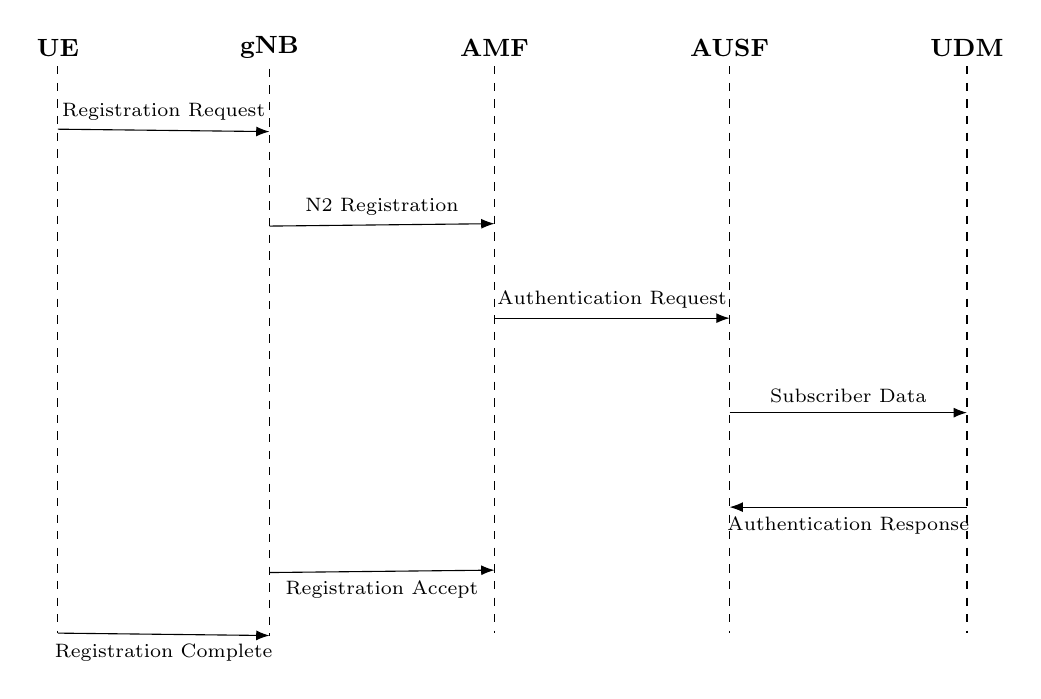
\begin{tikzpicture}[
		>=Latex,
		node distance=1cm,
		every node/.style={
			font=\small,
			align=center
		}
		]
		
		%--------------------------------------------------
		% Vertical Lifelines
		%--------------------------------------------------
		
		\node (ue)  {\textbf{UE}};
		\node (gnb) [right=1.8cm of ue] {\textbf{gNB}};
		\node (amf) [right=1.8cm of gnb] {\textbf{AMF}};
		\node (ausf)[right=1.8cm of amf] {\textbf{AUSF}};
		\node (udm) [right=1.8cm of ausf] {\textbf{UDM}};
		
		\foreach \x in {ue,gnb,amf,ausf,udm}
		{
			\draw[dashed] (\x.south) -- ++(0,-7.2);
		}
		
		%--------------------------------------------------
		% Messages
		%--------------------------------------------------
		
		\draw[->]
		($(ue.south)+(0,-0.8)$)
		--
		node[above,font=\scriptsize]{Registration Request}
		($(gnb.south)+(0,-0.8)$);
		
		\draw[->]
		($(gnb.south)+(0,-2.0)$)
		--
		node[above,font=\scriptsize]{N2 Registration}
		($(amf.south)+(0,-2.0)$);
		
		\draw[->]
		($(amf.south)+(0,-3.2)$)
		--
		node[above,font=\scriptsize]{Authentication Request}
		($(ausf.south)+(0,-3.2)$);
		
		\draw[->]
		($(ausf.south)+(0,-4.4)$)
		--
		node[above,font=\scriptsize]{Subscriber Data}
		($(udm.south)+(0,-4.4)$);
		
		\draw[<-]
		($(ausf.south)+(0,-5.6)$)
		--
		node[below,font=\scriptsize]{Authentication Response}
		($(udm.south)+(0,-5.6)$);
		
		\draw[<-]
		($(amf.south)+(0,-6.4)$)
		--
		node[below,font=\scriptsize]{Registration Accept}
		($(gnb.south)+(0,-6.4)$);
		
		\draw[<-]
		($(gnb.south)+(0,-7.2)$)
		--
		node[below,font=\scriptsize]{Registration Complete}
		($(ue.south)+(0,-7.2)$);
		
	\end{tikzpicture}
	
	\caption{Simplified 5G UE Registration Message Sequence.}
	\label{fig:registration_sequence}
	
\end{figure}
	
	%%%%%%%%%%%%%%%%%%%%%%%%%%%%%%%%%%%%%%%%%%%%%%%%%%%%%%%%%%%%
	
	\subsection{Phase II: PDU Session Establishment}
	
	Following successful authentication, the UE requests establishment of a Packet Data Unit (PDU) session. The AMF forwards the request to the Session Management Function (SMF), which allocates an IP address, selects an appropriate User Plane Function (UPF), and configures forwarding rules through the PFCP protocol.
	
	After successful tunnel establishment, GTP-U tunnels are created between the serving gNodeB and the UPF. User traffic can now reach external Data Networks through the N6 interface.
	
	The resulting communication path is illustrated in .
	
\begin{figure}[htbp]
	\centering
	
	\begin{tikzpicture}[
		>=Latex,
		every node/.style={
			font=\small,
			align=center
		}
		]
		
		%--------------------------------------------------
		% Lifelines
		%--------------------------------------------------
		
		\node (ue) {\textbf{UE}};
		\node (gnb) [right=1.7cm of ue] {\textbf{gNB}};
		\node (amf) [right=1.7cm of gnb] {\textbf{AMF}};
		\node (smf) [right=1.7cm of amf] {\textbf{SMF}};
		\node (upf) [right=1.7cm of smf] {\textbf{UPF}};
		\node (dn) [right=1.7cm of upf] {\textbf{Internet}};
		
		\foreach \x in {ue,gnb,amf,smf,upf,dn}
		{
			\draw[dashed] (\x.south) -- ++(0,-8.0);
		}
		
		%--------------------------------------------------
		% Messages
		%--------------------------------------------------
		
		\draw[->,blue,thick]
		($(ue.south)+(0,-0.8)$)
		--
		node[above,font=\scriptsize]{PDU Session Request}
		($(gnb.south)+(0,-0.8)$);
		
		\draw[->,blue,thick]
		($(gnb.south)+(0,-2.0)$)
		--
		node[above,font=\scriptsize]{N2}
		($(amf.south)+(0,-2.0)$);
		
		\draw[->,blue,thick]
		($(amf.south)+(0,-3.2)$)
		--
		node[above,font=\scriptsize]{Session Setup}
		($(smf.south)+(0,-3.2)$);
		
		\draw[->,blue,thick]
		($(smf.south)+(0,-4.4)$)
		--
		node[above,font=\scriptsize]{N4 (PFCP)}
		($(upf.south)+(0,-4.4)$);
		
		\draw[->,red,very thick]
		($(gnb.south)+(0,-5.8)$)
		--
		node[above,font=\scriptsize]{N3 (GTP-U)}
		($(upf.south)+(0,-5.8)$);
		
		\draw[->,red,very thick]
		($(upf.south)+(0,-7.0)$)
		--
		node[above,font=\scriptsize]{N6}
		($(dn.south)+(0,-7.0)$);
		
	\end{tikzpicture}
	
	\caption{Simplified PDU Session Establishment Procedure Showing Control and User Plane Interfaces.}
	\label{fig:pdu_flow}
	
\end{figure}
	
	%%%%%%%%%%%%%%%%%%%%%%%%%%%%%%%%%%%%%%%%%%%%%%%%%%%%%%%%%%%%
	
	\subsection{Phase III: Continuous Mobility Monitoring}
	
	Once connected, the UE continuously measures neighbouring cells using Reference Signal Received Power (RSRP), Reference Signal Received Quality (RSRQ), Signal-to-Interference-plus-Noise Ratio (SINR), and Channel Quality Indicator (CQI).
	
	These measurements are periodically transmitted to the serving gNodeB through Measurement Reports.
	
	The gNodeB forwards the collected measurements to the AMF, enabling the Core Network to evaluate whether a handover should be initiated.
	
	Within the proposed research platform, these measurement reports are simultaneously streamed to the AI Mobility Controller, where Deep Neural Networks and Reinforcement Learning models estimate future user trajectories and proactively prepare neighbouring cells before signal degradation occurs.
	
	%%%%%%%%%%%%%%%%%%%%%%%%%%%%%%%%%%%%%%%%%%%%%%%%%%%%%%%%%%%%
	
	\subsection{Phase IV: Intelligent Handover Procedure}
	
	Conventional 5G handover decisions are largely based on signal quality thresholds and hysteresis timers. Although effective for maintaining radio connectivity, these methods are unaware of network slice availability, edge computing load, application latency requirements, and future user movement.
	
	The proposed research introduces an AI-assisted mobility framework capable of evaluating multiple network parameters simultaneously before initiating a handover.
	
	The complete handover process is summarized below:
	
	\begin{enumerate}
		
		\item UE periodically transmits Measurement Reports.
		
		\item AI Mobility Controller predicts future trajectory.
		
		\item Candidate gNodeBs are ranked according to:
		
		\begin{itemize}
			
			\item Signal strength
			
			\item Slice availability
			
			\item MEC utilization
			
			\item Current traffic load
			
			\item Predicted congestion
			
			\item User QoS requirements
			
		\end{itemize}
		
		\item Target gNodeB resources are reserved.
		
		\item AMF initiates handover.
		
		\item SMF updates forwarding policies.
		
		\item UPF redirects GTP-U tunnels.
		
		\item UE synchronizes with the target gNodeB.
		
		\item Source gNodeB releases radio resources.
		
	\end{enumerate}
	
	%%%%%%%%%%%%%%%%%%%%%%%%%%%%%%%%%%%%%%%%%%%%%%%%%%%%%%%%%%%%
	
	\begin{figure}[h]
		
		\centering
		
		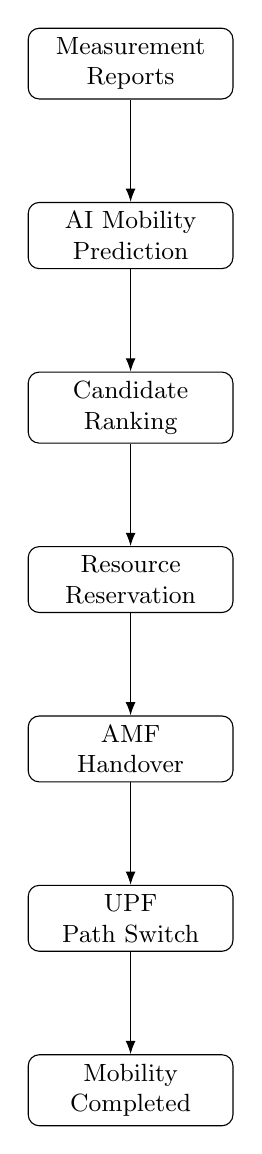
\begin{tikzpicture}[>=Latex,
			node distance=1.3cm,
			every node/.style={
				draw,
				rounded corners,
				minimum width=2.6cm,
				minimum height=0.7cm,
				align=center,
				font=\small}]
			
			\node (mr){Measurement\\Reports};
			
			\node (ai)[below=of mr]{AI Mobility\\Prediction};
			
			\node (rank)[below=of ai]{Candidate\\Ranking};
			
			\node (reserve)[below=of rank]{Resource\\Reservation};
			
			\node (handover)[below=of reserve]{AMF\\Handover};
			
			\node (switch)[below=of handover]{UPF\\Path Switch};
			
			\node (complete)[below=of switch]{Mobility\\Completed};
			
			\draw[->](mr)--(ai);
			
			\draw[->](ai)--(rank);
			
			\draw[->](rank)--(reserve);
			
			\draw[->](reserve)--(handover);
			
			\draw[->](handover)--(switch);
			
			\draw[->](switch)--(complete);
			
		\end{tikzpicture}
		
		\caption{AI-Assisted Intelligent Handover Procedure}
		
		\label{fig:handover_ai}
		
	\end{figure}
	
	%%%%%%%%%%%%%%%%%%%%%%%%%%%%%%%%%%%%%%%%%%%%%%%%%%%%%%%%%%%%
	
	\subsection{Preserving IP Continuity During Mobility}
	
	One of the principal objectives of this research is to preserve the UE's allocated IP address throughout inter-cell mobility. Since the User Plane Function (UPF) acts as the IP anchor within the 5G Core, changes in the serving gNodeB do not require IP reassignment.
	
	Instead, only the GTP-U forwarding tunnels are modified while maintaining the same logical IP session. Consequently, ongoing TCP sessions, multimedia streams, edge computing applications, and network slice contexts remain uninterrupted during mobility.
	
	The proposed AI framework further reduces handover interruption time by proactively configuring forwarding paths before the UE reaches the target cell, thereby minimizing packet loss, latency spikes, and service disruption.
	
	%%%%%%%%%%%%%%%%%%%%%%%%%%%%%%%%%%%%%%%%%%%%%%%%%%%%%%%%%%%%%%%%%%%%%%%%%%%%%%%%%%
	\section{AI-Assisted Mobility Management Framework}
	
	Conventional mobility management algorithms defined by the 3GPP specifications primarily rely upon radio measurements such as the Reference Signal Received Power (RSRP), Reference Signal Received Quality (RSRQ), Signal-to-Interference-plus-Noise Ratio (SINR), and configurable hysteresis timers. While these approaches are effective for maintaining basic radio connectivity, they remain unaware of higher-layer network conditions including edge server utilization, slice availability, Quality of Service (QoS) requirements, traffic congestion, and predicted user trajectories.
	
	Consequently, users may be handed over to geographically closer cells that are already overloaded, lack the required network slice resources, or host heavily loaded edge computing servers. Such decisions often lead to unnecessary packet loss, increased latency, degraded Quality of Experience (QoE), and frequent handover failures.
	
	The proposed research introduces an Artificial Intelligence assisted mobility framework capable of integrating radio measurements with network-wide telemetry to perform predictive and context-aware mobility management.
	
	%%%%%%%%%%%%%%%%%%%%%%%%%%%%%%%%%%%%%%%%%%%%%%%%%%%%%%%%%%%%%%%
	
	\subsection{Overall AI Decision Pipeline}
	
	The proposed framework continuously collects measurements from multiple layers of the network.
	
	\begin{itemize}
		
		\item User Equipment (UE) radio measurements
		
		\item gNodeB scheduling statistics
		
		\item Core Network signaling events
		
		\item User Plane traffic statistics
		
		\item Edge Computing resource utilization
		
		\item Network Slice resource allocation
		
		\item Historical mobility traces
		
	\end{itemize}
	
	These heterogeneous data streams are synchronized and processed by a centralized AI Mobility Controller responsible for predicting future network conditions and selecting the optimal target cell before conventional threshold-based handover algorithms are triggered.
	
	%%%%%%%%%%%%%%%%%%%%%%%%%%%%%%%%%%%%%%%%%%%%%%%%%%%%%%%%%%%%%%%
	
	\begin{figure}[h]
		
		\centering
		
		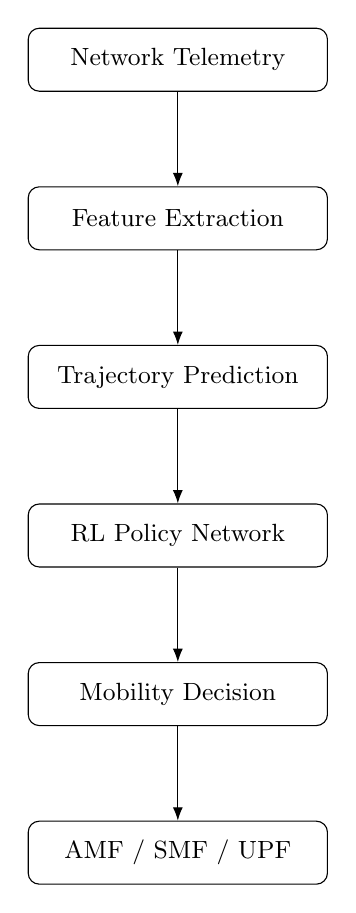
\begin{tikzpicture}[>=Latex,
			node distance=1.2cm,
			every node/.style={
				draw,
				rounded corners,
				minimum width=3.8cm,
				minimum height=0.8cm,
				align=center,
				font=\small
			}]
			
			\node (collect){Network Telemetry};
			
			\node (feature)[below=of collect]{Feature Extraction};
			
			\node (predict)[below=of feature]{Trajectory Prediction};
			
			\node (policy)[below=of predict]{RL Policy Network};
			
			\node (decision)[below=of policy]{Mobility Decision};
			
			\node (execute)[below=of decision]{AMF / SMF / UPF};
			
			\draw[->](collect)--(feature);
			
			\draw[->](feature)--(predict);
			
			\draw[->](predict)--(policy);
			
			\draw[->](policy)--(decision);
			
			\draw[->](decision)--(execute);
			
		\end{tikzpicture}
		
		\caption{Overall AI-Assisted Mobility Decision Pipeline}
		
		\label{fig:ai_pipeline}
		
	\end{figure}
	
	%%%%%%%%%%%%%%%%%%%%%%%%%%%%%%%%%%%%%%%%%%%%%%%%%%%%%%%%%%%%%%%
	
	\subsection{Feature Collection}
	
	Unlike conventional mobility algorithms that only utilize signal strength, the proposed framework constructs a high-dimensional feature vector by aggregating measurements from multiple network entities.
	
	The collected parameters include
	
	\begin{table}[h]
		
		\centering
		
		\caption{Input Features Used by the AI Mobility Controller}
		
		\label{tab:features}
		
		\begin{tabular}{p{4cm}p{9cm}}
			
			\toprule
			
			\textbf{Category}
			
			&
			
			\textbf{Collected Parameters}
			
			\\
			
			\midrule
			
			Radio Measurements
			
			&
			
			RSRP, RSRQ, SINR, CQI, BLER
			
			\\
			
			Mobility
			
			&
			
			Velocity, Direction, GPS Coordinates, Cell Residence Time
			
			\\
			
			Core Network
			
			&
			
			AMF Load, SMF Load, Active Sessions
			
			\\
			
			User Plane
			
			&
			
			Throughput, Packet Delay, Packet Loss, Jitter
			
			\\
			
			Edge Computing
			
			&
			
			CPU Utilization, GPU Utilization, Memory Usage
			
			\\
			
			Network Slicing
			
			&
			
			Slice Availability, Slice Utilization, Reserved Resources
			
			\\
			
			Historical Data
			
			&
			
			Past Mobility Patterns, Previous Handover Success Rate
			
			\\
			
			\bottomrule
			
		\end{tabular}
		
	\end{table}
	
	%%%%%%%%%%%%%%%%%%%%%%%%%%%%%%%%%%%%%%%%%%%%%%%%%%%%%%%%%%%%%%%
	
	\subsection{Prediction Module}
	
	The prediction engine estimates the future state of the network several seconds ahead.
	
	Instead of reacting after signal degradation has already occurred, the AI controller predicts
	
	\begin{itemize}
		
		\item Future UE trajectory
		
		\item Future serving cell
		
		\item Expected signal quality
		
		\item Candidate gNodeB load
		
		\item Slice availability
		
		\item MEC server congestion
		
		\item Network latency
		
		\item Probability of handover failure
		
	\end{itemize}
	
	These predictions enable proactive preparation of neighboring cells before the UE physically reaches the cell boundary.
	
	%%%%%%%%%%%%%%%%%%%%%%%%%%%%%%%%%%%%%%%%%%%%%%%%%%%%%%%%%%%%%%%
	
	\subsection{Reinforcement Learning Based Decision Engine}
	
	A Deep Reinforcement Learning (DRL) agent continuously interacts with the network environment to determine the optimal mobility action.
	
	The state space consists of the complete network feature vector collected from the Radio Access Network, Core Network, and Edge Computing infrastructure.
	
	The action space includes
	
	\begin{itemize}
		
		\item Maintain current serving cell
		
		\item Trigger handover
		
		\item Delay handover
		
		\item Reserve neighboring resources
		
		\item Switch Network Slice
		
		\item Migrate MEC application
		
		\item Modify QoS policy
		
	\end{itemize}
	
	The reward function is designed to maximize
	
	\begin{itemize}
		
		\item Successful handovers
		
		\item End-to-end throughput
		
		\item Slice utilization
		
		\item User Quality of Experience (QoE)
		
	\end{itemize}
	
	while minimizing
	
	\begin{itemize}
		
		\item Packet loss
		
		\item Latency
		
		\item Ping-pong handovers
		
		\item Energy consumption
		
		\item Signaling overhead
		
	\end{itemize}
	
	%%%%%%%%%%%%%%%%%%%%%%%%%%%%%%%%%%%%%%%%%%%%%%%%%%%%%%%%%%%%%%%
	
	\subsection{Closed Loop Network Optimization}
	
	Unlike traditional reactive mobility management, the proposed framework forms a continuous feedback loop.
	
\begin{figure}[htbp]
	\centering
	
	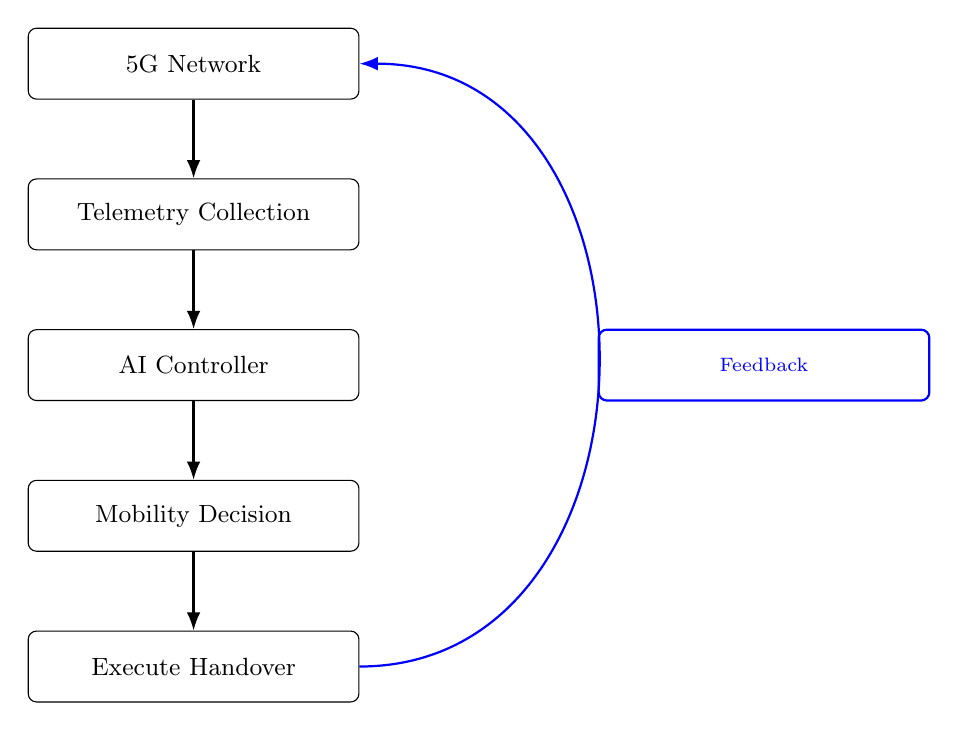
\begin{tikzpicture}[
		>=Latex,
		node distance=1.5cm,
		every node/.style={
			draw,
			rounded corners=3pt,
			minimum width=4.2cm,
			minimum height=0.9cm,
			align=center,
			font=\small
		}
		]
		
		%--------------------------------------------------
		% Nodes
		%--------------------------------------------------
		
		\node (network) {5G Network};
		
		\node (telemetry) [below=1.0cm of network]
		{Telemetry Collection};
		
		\node (ai) [below=1.0cm of telemetry]
		{AI Controller};
		
		\node (decision) [below=1.0cm of ai]
		{Mobility Decision};
		
		\node (execute) [below=1.0cm of decision]
		{Execute Handover};
		
		%--------------------------------------------------
		% Forward Flow
		%--------------------------------------------------
		
		\draw[->,thick]
		(network) -- (telemetry);
		
		\draw[->,thick]
		(telemetry) -- (ai);
		
		\draw[->,thick]
		(ai) -- (decision);
		
		\draw[->,thick]
		(decision) -- (execute);
		
		%--------------------------------------------------
		% Feedback Loop
		%--------------------------------------------------
		
		\draw[->,thick,blue]
		(execute.east)
		to[out=0,in=0,looseness=1.35]
		node[right,font=\scriptsize]{Feedback}
		(network.east);
		
	\end{tikzpicture}
	
	\caption{Closed-Loop AI Mobility Optimization Framework.}
	\label{fig:closed_loop}
	
\end{figure}
	
	\section{Experimental Methodology and Evaluation Framework}
	
	The primary objective of the proposed testbed is to experimentally evaluate Artificial Intelligence assisted mobility management algorithms under realistic 5G Standalone deployment scenarios. Unlike simulation-only studies, the proposed infrastructure enables controlled experimentation over real radio hardware, commercial User Equipments (UEs), physical servers, and software-defined radio base stations.
	
	The evaluation methodology has been designed to ensure reproducibility, statistical significance, and objective comparison against conventional 3GPP mobility management algorithms.
	
	%%%%%%%%%%%%%%%%%%%%%%%%%%%%%%%%%%%%%%%%%%%%%%%%%%%%%%%%%%%%%%%%%%%%%%
	
	\subsection{Experimental Workflow}
	
	Each experiment follows a standardized workflow beginning with network initialization and ending with statistical performance analysis.
	
	\vspace{0.3cm}
	
	\begin{figure}[h]
		
		\centering
		
		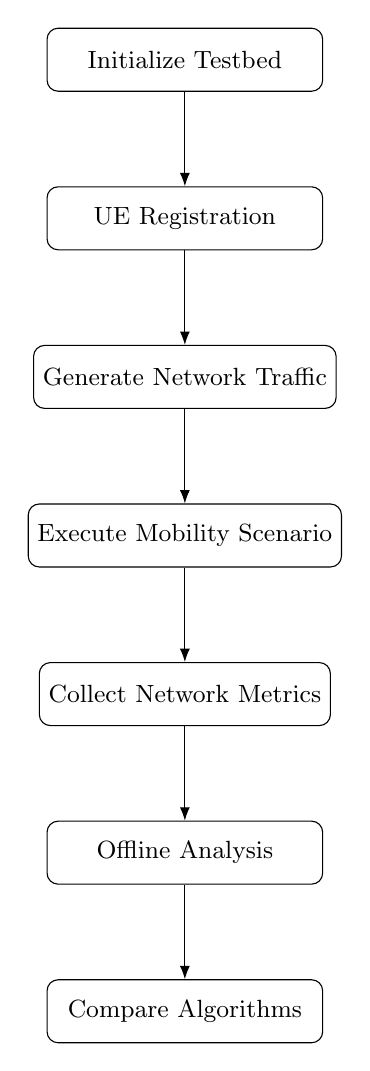
\begin{tikzpicture}[>=Latex,
			node distance=1.2cm,
			every node/.style={
				draw,
				rounded corners,
				minimum width=3.5cm,
				minimum height=0.8cm,
				align=center,
				font=\small
			}]
			
			\node (init){Initialize Testbed};
			
			\node (register)[below=of init]{UE Registration};
			
			\node (traffic)[below=of register]{Generate Network Traffic};
			
			\node (mobility)[below=of traffic]{Execute Mobility Scenario};
			
			\node (collect)[below=of mobility]{Collect Network Metrics};
			
			\node (analysis)[below=of collect]{Offline Analysis};
			
			\node (compare)[below=of analysis]{Compare Algorithms};
			
			\draw[->](init)--(register);
			
			\draw[->](register)--(traffic);
			
			\draw[->](traffic)--(mobility);
			
			\draw[->](mobility)--(collect);
			
			\draw[->](collect)--(analysis);
			
			\draw[->](analysis)--(compare);
			
		\end{tikzpicture}
		
		\caption{Overall Experimental Workflow}
		
		\label{fig:workflow}
		
	\end{figure}
	
	%%%%%%%%%%%%%%%%%%%%%%%%%%%%%%%%%%%%%%%%%%%%%%%%%%%%%%%%%%%%%%%%%%%%%%
	
	\subsection{Baseline Mobility Algorithms}
	
	The proposed AI framework will be compared against conventional mobility management techniques implemented within current 3GPP-compliant cellular systems.
	
	The following baseline algorithms will be evaluated.
	
	\begin{table}[h]
		
		\centering
		
		\caption{Baseline Algorithms}
		
		\begin{tabular}{p{5cm}p{9cm}}
			
			\toprule
			
			Algorithm
			
			&
			
			Description
			
			\\
			
			\midrule
			
			RSRP Based Handover
			
			&
			
			Conventional strongest-signal selection.
			
			\\
			
			RSRP + Hysteresis
			
			&
			
			Standard LTE/5G implementation using configurable hysteresis margins.
			
			\\
			
			A3 Event Trigger
			
			&
			
			3GPP Event A3 mobility procedure.
			
			\\
			
			Time-to-Trigger (TTT)
			
			&
			
			Threshold-based delayed handover.
			
			\\
			
			Proposed AI Mobility
			
			&
			
			Deep Reinforcement Learning assisted predictive mobility management.
			
			\\
			
			\bottomrule
			
		\end{tabular}
		
	\end{table}
	
	%%%%%%%%%%%%%%%%%%%%%%%%%%%%%%%%%%%%%%%%%%%%%%%%%%%%%%%%%%%%%%%%%%%%%%
	
	\subsection{Mobility Scenarios}
	
	To evaluate algorithm robustness under varying operating conditions, multiple mobility scenarios will be investigated.
	
	\begin{table}[h]
		
		\centering
		
		\caption{Mobility Test Scenarios}
		
		\begin{tabular}{p{5cm}p{8cm}c}
			
			\toprule
			
			Scenario
			
			&
			
			Description
			
			&
			
			Velocity
			
			\\
			
			\midrule
			
			Pedestrian
			
			&
			
			Walking user
			
			&
			
			3--5 km/h
			
			\\
			
			Cyclist
			
			&
			
			Campus mobility
			
			&
			
			15 km/h
			
			\\
			
			Vehicle
			
			&
			
			Urban road
			
			&
			
			30--60 km/h
			
			\\
			
			High Speed
			
			&
			
			Fast moving UE
			
			&
			
			80--120 km/h
			
			\\
			
			Dense Cell
			
			&
			
			Frequent handovers
			
			&
			
			Variable
			
			\\
			
			\bottomrule
			
		\end{tabular}
		
	\end{table}
	
	%%%%%%%%%%%%%%%%%%%%%%%%%%%%%%%%%%%%%%%%%%%%%%%%%%%%%%%%%%%%%%%%%%%%%%
	
	\subsection{Traffic Profiles}
	
	The network will be subjected to multiple application workloads representative of practical deployments.
	
	\begin{itemize}
		
		\item UHD Video Streaming
		
		\item VoNR Voice Calls
		
		\item Web Browsing
		
		\item IoT Telemetry
		
		\item MEC Video Analytics
		
		\item Large File Transfer
		
		\item Mixed Enterprise Traffic
		
	\end{itemize}
	
	%%%%%%%%%%%%%%%%%%%%%%%%%%%%%%%%%%%%%%%%%%%%%%%%%%%%%%%%%%%%%%%%%%%%%%
	
	\subsection{Performance Metrics}
	
	Each experiment will record both radio-level and network-level performance indicators.
	
	\begin{table}[h]
		
		\centering
		
		\caption{Evaluation Metrics}
		
		\begin{tabular}{p{5cm}p{8cm}}
			
			\toprule
			
			Metric
			
			&
			
			Purpose
			
			\\
			
			\midrule
			
			Handover Delay
			
			&
			
			Time required to complete mobility.
			
			\\
			
			Packet Loss
			
			&
			
			Packets dropped during mobility.
			
			\\
			
			Latency
			
			&
			
			End-to-end network delay.
			
			\\
			
			Jitter
			
			&
			
			Variation in packet delay.
			
			\\
			
			Throughput
			
			&
			
			Application data rate.
			
			\\
			
			RSRP
			
			&
			
			Signal strength.
			
			\\
			
			SINR
			
			&
			
			Signal quality.
			
			\\
			
			CQI
			
			&
			
			Channel quality.
			
			\\
			
			Slice Utilization
			
			&
			
			Resource utilization.
			
			\\
			
			MEC Response Time
			
			&
			
			Application latency.
			
			\\
			
			CPU Usage
			
			&
			
			Core server utilization.
			
			\\
			
			GPU Usage
			
			&
			
			AI inference workload.
			
			\\
			
			Power Consumption
			
			&
			
			Energy efficiency.
			
			\\
			
			\bottomrule
			
		\end{tabular}
		
	\end{table}
	
	%%%%%%%%%%%%%%%%%%%%%%%%%%%%%%%%%%%%%%%%%%%%%%%%%%%%%%%%%%%%%%%%%%%%%%
	
	\subsection{Data Collection Pipeline}
	
	Experimental measurements will be collected simultaneously from multiple infrastructure components.
	
	\begin{figure}[h]
		
		\centering
		
		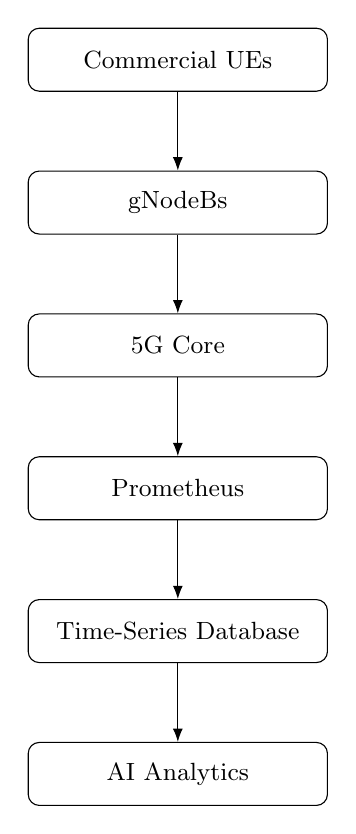
\begin{tikzpicture}[>=Latex,
			node distance=1cm,
			every node/.style={
				draw,
				rounded corners,
				minimum width=3.8cm,
				minimum height=0.8cm,
				align=center,
				font=\small
			}]
			
			\node (ue){Commercial UEs};
			
			\node (gnb)[below=of ue]{gNodeBs};
			
			\node (core)[below=of gnb]{5G Core};
			
			\node (telemetry)[below=of core]{Prometheus};
			
			\node (storage)[below=of telemetry]{Time-Series Database};
			
			\node (analysis)[below=of storage]{AI Analytics};
			
			\draw[->](ue)--(gnb);
			
			\draw[->](gnb)--(core);
			
			\draw[->](core)--(telemetry);
			
			\draw[->](telemetry)--(storage);
			
			\draw[->](storage)--(analysis);
			
		\end{tikzpicture}
		
		\caption{Experimental Data Collection Pipeline}
		
		\label{fig:data_pipeline}
		
	\end{figure}
	
	%%%%%%%%%%%%%%%%%%%%%%%%%%%%%%%%%%%%%%%%%%%%%%%%%%%%%%%%%%%%%%%%%%%%%%
	
	\subsection{Statistical Analysis}
	
	Each experiment will be repeated multiple times to eliminate random fluctuations caused by radio propagation, operating system scheduling, and wireless interference.
	
	The collected measurements will be statistically analyzed using
	
	\begin{itemize}
		
		\item Mean
		
		\item Median
		
		\item Standard Deviation
		
		\item Confidence Interval
		
		\item Box Plots
		
		\item Cumulative Distribution Function (CDF)
		
		\item One-way ANOVA
		
		\item Paired t-test
		
	\end{itemize}
	
	Only statistically significant improvements will be considered valid research outcomes.
	
	%%%%%%%%%%%%%%%%%%%%%%%%%%%%%%%%%%%%%%%%%%%%%%%%%%%%%%%%%%%%%%%%%%%%%%
	
	\subsection{Expected Deliverables}
	
	The proposed experimental campaign is expected to generate
	
	\begin{itemize}
		
		\item Large-scale mobility datasets
		
		\item AI-ready training datasets
		
		\item Open-source mobility framework
		
		\item Performance benchmark reports
		
		\item Conference publications
		
		\item Journal publications
		
		\item Technology demonstrators
		
		\item Potential patent filings
		
	\end{itemize}
	
	The resulting datasets and performance evaluations will provide quantitative evidence of the effectiveness of AI-assisted mobility management under realistic deployment conditions.
	
	%%%%%%%%%%%%%%%%%%%%%%%%%%%%%%%%%%%%%%%%%%%%%%%%%%%%%%%%%%%%%%%%%%%%%%%%%%%%%%%%%%
	\section{Laboratory Infrastructure and Physical Deployment Design}
	
	The proposed research facility is designed as a compact private 5G Standalone laboratory capable of supporting realistic mobility experiments involving multiple radio cells, commercial User Equipments (UEs), edge computing servers, AI-assisted mobility controllers, and a standards-compliant 5G Core Network.
	
	Unlike purely software-based simulators, the proposed deployment incorporates physical Software Defined Radios (SDRs), dedicated compute servers, commercial networking equipment, and programmable User Equipments to accurately reproduce real-world radio propagation, network latency, and mobility behaviour.
	
	The laboratory is organized into five major infrastructure layers:
	
	\begin{enumerate}
		
		\item Core Network Infrastructure
		
		\item Radio Access Network (RAN)
		
		\item Edge Computing Infrastructure
		
		\item AI and Monitoring Infrastructure
		
		\item Network Backbone and Power Distribution
		
	\end{enumerate}
	
	%%%%%%%%%%%%%%%%%%%%%%%%%%%%%%%%%%%%%%%%%%%%%%%%%%%%%%%%%%%%%%%
	
	\subsection{Overall Laboratory Architecture}
	
	 illustrates the complete laboratory deployment.
	
	\begin{figure}[h]
		
		\centering
		
		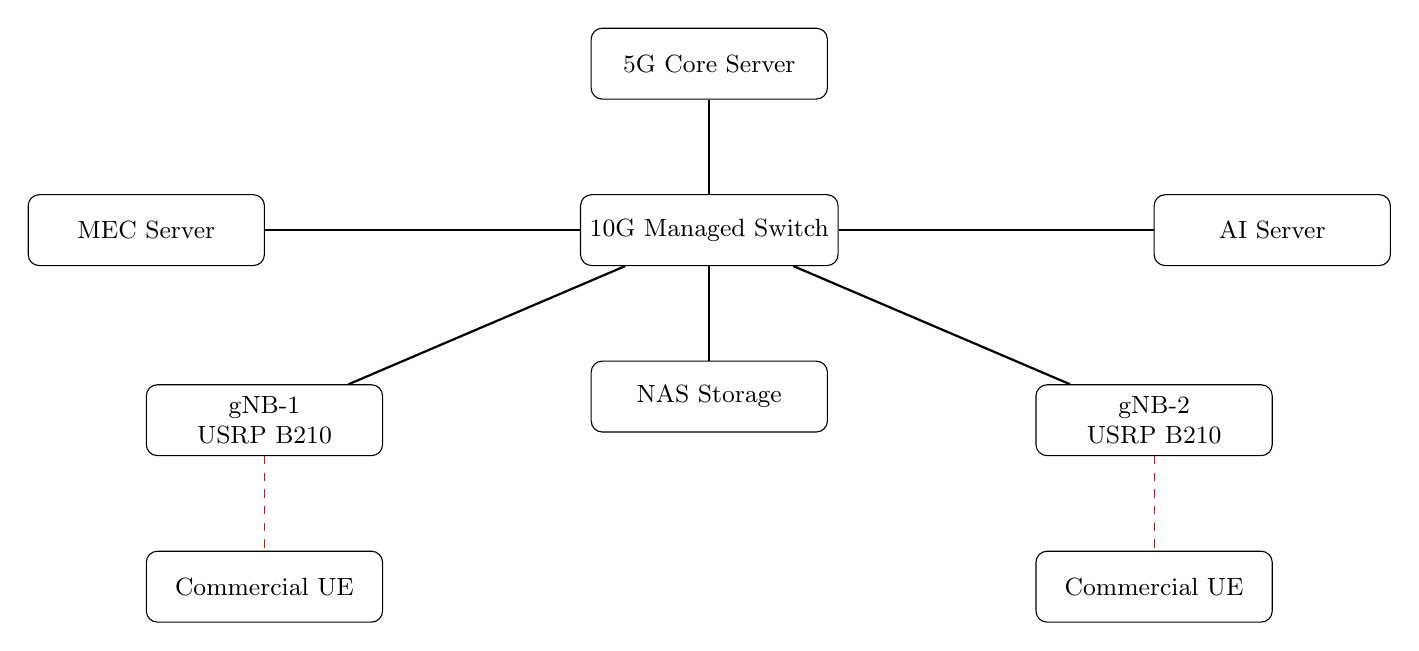
\begin{tikzpicture}[node distance=1.2cm,
			>=Latex,
			every node/.style={
				draw,
				rounded corners,
				align=center,
				minimum width=3cm,
				minimum height=0.9cm,
				font=\small
			}]
			
			\node(core){5G Core Server};
			
			\node(switch)[below=of core]{10G Managed Switch};
			
			\node(gnb1)[below left=1.5cm and 2.5cm of switch]{gNB-1\\USRP B210};
			
			\node(gnb2)[below right=1.5cm and 2.5cm of switch]{gNB-2\\USRP B210};
			
			\node(ai)[right=4cm of switch]{AI Server};
			
			\node(mec)[left=4cm of switch]{MEC Server};
			
			\node(nas)[below=of switch]{NAS Storage};
			
			\node(ue1)[below=of gnb1]{Commercial UE};
			
			\node(ue2)[below=of gnb2]{Commercial UE};
			
			\draw[thick](core)--(switch);
			
			\draw[thick](switch)--(gnb1);
			
			\draw[thick](switch)--(gnb2);
			
			\draw[thick](switch)--(mec);
			
			\draw[thick](switch)--(ai);
			
			\draw[thick](switch)--(nas);
			
			\draw[dashed,red](gnb1)--(ue1);
			
			\draw[dashed,red](gnb2)--(ue2);
			
		\end{tikzpicture}
		
		\caption{Overall Laboratory Infrastructure}
		
		\label{fig:lab_overview}
		
	\end{figure}
	
	%%%%%%%%%%%%%%%%%%%%%%%%%%%%%%%%%%%%%%%%%%%%%%%%%%%%%%%%%%%%%%%
	
	\subsection{Hardware Rack Organization}
	
	To improve maintainability, thermal management, and cable routing, all compute equipment will be installed within a standard 42U server rack.
	
	The proposed rack layout is shown in .
	
	\begin{figure}[h]
		
		\centering
		
		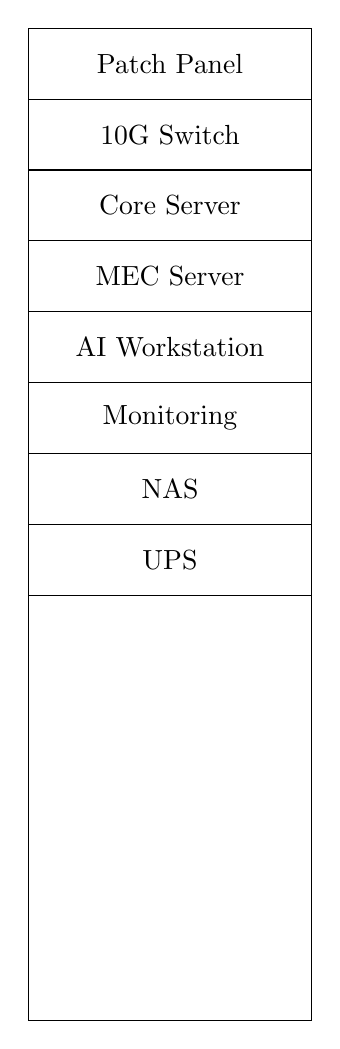
\begin{tikzpicture}[scale=0.9]
			
			\draw (0,0) rectangle (4,14);
			
			\foreach \y/\label in {
				13/{Patch Panel},
				12/{10G Switch},
				11/{Core Server},
				10/{MEC Server},
				9/{AI Workstation},
				8/{Monitoring},
				7/{NAS},
				6/{UPS}
			}
			{
				\draw (0,\y) rectangle (4,\y+1);
				\node at (2,\y+0.5){\label};
			}
			
		\end{tikzpicture}
		
		\caption{Proposed Server Rack Organization}
		
		\label{fig:rack_layout}
		
	\end{figure}
	
	%%%%%%%%%%%%%%%%%%%%%%%%%%%%%%%%%%%%%%%%%%%%%%%%%%%%%%%%%%%%%%%
	
	\subsection{Radio Access Network Deployment}
	
	The Radio Access Network consists of two Software Defined Radio based gNodeBs positioned to create overlapping coverage regions. This arrangement enables continuous mobility experiments involving inter-cell handovers.
	
	Each gNodeB comprises
	
	\begin{itemize}
		
		\item Ettus USRP B210 SDR
		
		\item Dedicated Host Computer
		
		\item External MIMO Antennas
		
		\item GPSDO (optional future upgrade)
		
		\item RF Attenuators for indoor testing
		
	\end{itemize}
	
	The overlapping coverage enables controlled execution of
	
	\begin{itemize}
		
		\item Intra-frequency handover
		
		\item Inter-cell mobility
		
		\item Slice migration
		
		\item Edge service migration
		
		\item Packet loss analysis
		
	\end{itemize}
	
	%%%%%%%%%%%%%%%%%%%%%%%%%%%%%%%%%%%%%%%%%%%%%%%%%%%%%%%%%%%%%%%
	
	\subsection{UE Mobility Corridor}
	
	To reproduce realistic mobility, a dedicated experimental corridor will be established inside the laboratory.
	
	\begin{figure}[h]
		
		\centering
		
		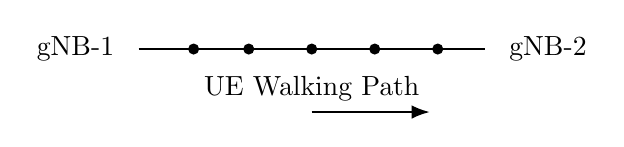
\begin{tikzpicture}[>=Latex]
			
			\node at (-3,0){gNB-1};
			
			\node at (3,0){gNB-2};
			
			\draw[thick](-2.2,0)--(2.2,0);
			
			\foreach \x in {-1.5,-0.8,0,0.8,1.6}
			{
				\fill (\x,0) circle (2pt);
			}
			
			\node at (0,-0.5){UE Walking Path};
			
			\draw[->,thick](0,-0.8)--(1.5,-0.8);
			
		\end{tikzpicture}
		
		\caption{Indoor Mobility Corridor}
		
		\label{fig:mobility_corridor}
		
	\end{figure}
	
	The mobility corridor enables repeatable experiments at controlled pedestrian speeds while ensuring identical trajectories across multiple experimental trials.
	
	%%%%%%%%%%%%%%%%%%%%%%%%%%%%%%%%%%%%%%%%%%%%%%%%%%%%%%%%%%%%%%%
	
	\subsection{Network Backbone}
	
	All infrastructure components communicate through a centralized Layer-2/Layer-3 managed switch supporting both Gigabit Ethernet and 10 Gigabit SFP+ uplinks.
	
	The proposed backbone supports
	
	\begin{itemize}
		
		\item 10 Gbps Core Server connectivity
		
		\item MEC communication
		
		\item NAS storage
		
		\item Monitoring traffic
		
		\item AI telemetry
		
		\item SDR host computers
		
	\end{itemize}
	
	This architecture minimizes bottlenecks during high-throughput mobility experiments.
	
	%%%%%%%%%%%%%%%%%%%%%%%%%%%%%%%%%%%%%%%%%%%%%%%%%%%%%%%%%%%%%%%
	
	\subsection{Power and Cooling Infrastructure}
	
	Continuous operation of the testbed requires reliable electrical and thermal management.
	
	The laboratory includes
	
	\begin{itemize}
		
		\item 5 kVA Online UPS
		
		\item Rack-mounted Power Distribution Unit
		
		\item Surge Protection
		
		\item Active Rack Cooling
		
		\item Dedicated Air Conditioning
		
		\item Automatic Shutdown Scripts
		
	\end{itemize}
	
	These provisions ensure uninterrupted execution of long-duration experiments and protect critical infrastructure against power failures.
	
	%%%%%%%%%%%%%%%%%%%%%%%%%%%%%%%%%%%%%%%%%%%%%%%%%%%%%%%%%%%%%%%
	
	\subsection{Future Expansion Capability}
	
	Although initially designed as a two-cell deployment, the proposed infrastructure has been intentionally over-engineered to accommodate future research activities.
	
	The laboratory can be expanded to support
	
	\begin{itemize}
		
		\item Four or more SDR-based gNodeBs
		
		\item Open RAN deployments
		
		\item O-RAN Near-RT RIC
		
		\item Multi-UPF architectures
		
		\item Additional MEC clusters
		
		\item AI-native 6G experimentation
		
		\item Satellite Non-Terrestrial Networks (NTN)
		
		\item Large-scale Network Slice orchestration
		
	\end{itemize}
	
	Consequently, the proposed laboratory serves not only the objectives of the current research project but also establishes a long-term experimental platform for future wireless communication research.
	
	%%%%%%%%%%%%%%%%%%%%%%%%%%%%%%%%%%%%%%%%%%%%%%%%%%%%%%%%%%%%%%%%%%%%%%%%%%%%%%%%%%
	\section{Research Objectives and Planned Experimental Campaign}
	
	The establishment of the proposed 5G Standalone research testbed enables a comprehensive investigation into intelligent mobility management, AI-assisted network slicing, and edge-aware service orchestration under realistic deployment conditions. Rather than serving solely as an infrastructure project, the laboratory has been designed to facilitate long-term experimental research aligned with current challenges in beyond-5G (B5G) and emerging 6G communication systems.
	
	The experimental campaign is organized into multiple research themes, each targeting a specific aspect of intelligent mobility management and network optimization.
	
	%%%%%%%%%%%%%%%%%%%%%%%%%%%%%%%%%%%%%%%%%%%%%%%%%%%%%%%%%%%%%%%%%%%%%%%%%%%%%%%
	
	\subsection{Research Objective 1: Intelligent Mobility Prediction}
	
	The first objective focuses on predicting future user mobility before conventional handover triggers are activated.
	
	Current cellular systems initiate handovers only after radio signal quality begins to degrade. Such reactive mechanisms often lead to increased packet loss, unnecessary signaling, and temporary degradation in Quality of Service (QoS).
	
	The proposed research investigates machine learning models capable of predicting
	
	\begin{itemize}
		
		\item Future user trajectory
		
		\item Future serving cell
		
		\item Expected signal quality
		
		\item Probability of handover
		
		\item Time until handover
		
	\end{itemize}
	
	These predictions enable proactive resource reservation and intelligent mobility planning.
	
	%%%%%%%%%%%%%%%%%%%%%%%%%%%%%%%%%%%%%%%%%%%%%%%%%%%%%%%%%%%%%%%%%%%%%%%%%%%%%%%
	
	\subsection{Research Objective 2: AI-Assisted Handover Optimization}
	
	The second research objective evaluates reinforcement learning algorithms capable of dynamically selecting the optimal target cell.
	
	Unlike traditional strongest-signal approaches, the proposed framework simultaneously considers
	
	\begin{itemize}
		
		\item Radio signal quality
		
		\item Cell congestion
		
		\item Available bandwidth
		
		\item Edge server utilization
		
		\item Network slice availability
		
		\item Historical mobility information
		
		\item User Quality of Experience
		
	\end{itemize}
	
	The effectiveness of the proposed decision framework will be evaluated against standard 3GPP handover algorithms.
	
	%%%%%%%%%%%%%%%%%%%%%%%%%%%%%%%%%%%%%%%%%%%%%%%%%%%%%%%%%%%%%%%%%%%%%%%%%%%%%%%
	
	\subsection{Research Objective 3: Intelligent Network Slice Selection}
	
	Network slicing represents one of the defining technologies of fifth-generation communication systems.
	
	Instead of assigning users to static slices, this work investigates adaptive slice allocation strategies capable of responding to changing network conditions.
	
	The proposed AI controller continuously evaluates
	
	\begin{itemize}
		
		\item Slice utilization
		
		\item SLA compliance
		
		\item User application requirements
		
		\item Available radio resources
		
		\item Edge computing availability
		
	\end{itemize}
	
	before selecting the most appropriate slice instance.
	
	%%%%%%%%%%%%%%%%%%%%%%%%%%%%%%%%%%%%%%%%%%%%%%%%%%%%%%%%%%%%%%%%%%%%%%%%%%%%%%%
	
	\subsection{Research Objective 4: Edge Service Continuity}
	
	Modern low-latency applications frequently execute on Multi-access Edge Computing (MEC) servers.
	
	During mobility, users may move away from the serving MEC node, increasing application latency.
	
	This research investigates
	
	\begin{itemize}
		
		\item Dynamic edge service migration
		
		\item Container relocation
		
		\item Service redirection
		
		\item Traffic steering
		
		\item Edge resource prediction
		
	\end{itemize}
	
	to maintain uninterrupted application performance throughout mobility.
	
	%%%%%%%%%%%%%%%%%%%%%%%%%%%%%%%%%%%%%%%%%%%%%%%%%%%%%%%%%%%%%%%%%%%%%%%%%%%%%%%
	
	\subsection{Research Objective 5: Energy-Efficient Mobility Management}
	
	In addition to maximizing Quality of Service, future communication networks must reduce infrastructure energy consumption.
	
	The proposed framework investigates energy-aware mobility decisions considering
	
	\begin{itemize}
		
		\item Base station utilization
		
		\item Computational load
		
		\item Network traffic
		
		\item AI inference overhead
		
		\item Power consumption of SDR infrastructure
		
	\end{itemize}
	
	The resulting algorithms are expected to improve both network performance and operational efficiency.
	
	%%%%%%%%%%%%%%%%%%%%%%%%%%%%%%%%%%%%%%%%%%%%%%%%%%%%%%%%%%%%%%%%%%%%%%%%%%%%%%%
	
	\subsection{Experimental Campaign}
	
	The experimental evaluation will be divided into multiple phases as summarized in Table~\ref{tab}.
	
	\begin{table}[h]
		
		\centering
		
		\caption{Planned Experimental Campaign}
		
		\label{tab:campaign}
		
		\begin{tabular}{p{3cm}p{9cm}}
			
			\toprule
			
			Phase
			
			&
			
			Objective
			
			\\
			
			\midrule
			
			Phase I
			
			&
			
			Deployment and validation of the private 5G Standalone network.
			
			\\
			
			Phase II
			
			&
			
			Baseline mobility experiments using standard 3GPP algorithms.
			
			\\
			
			Phase III
			
			&
			
			Collection of mobility telemetry datasets.
			
			\\
			
			Phase IV
			
			&
			
			Training of Deep Learning and Reinforcement Learning models.
			
			\\
			
			Phase V
			
			&
			
			Deployment of AI-assisted mobility controller.
			
			\\
			
			Phase VI
			
			&
			
			Comparative evaluation under multiple mobility scenarios.
			
			\\
			
			Phase VII
			
			&
			
			Scalability analysis involving increasing numbers of users and cells.
			
			\\
			
			Phase VIII
			
			&
			
			Publication, dataset release, and technology demonstration.
			
			\\
			
			\bottomrule
			
		\end{tabular}
		
	\end{table}
	
	%%%%%%%%%%%%%%%%%%%%%%%%%%%%%%%%%%%%%%%%%%%%%%%%%%%%%%%%%%%%%%%%%%%%%%%%%%%%%%%
	
	\subsection{Expected Scientific Contributions}
	
	The proposed research is expected to contribute
	
	\begin{itemize}
		
		\item AI-assisted mobility management algorithms.
		
		\item Reinforcement learning based handover optimization.
		
		\item Dynamic network slice selection framework.
		
		\item Edge-aware mobility orchestration.
		
		\item Large-scale real-world mobility datasets.
		
		\item Benchmark datasets for future wireless communication research.
		
		\item Open-source software components.
		
		\item Publications in IEEE Transactions, Elsevier, and Springer journals.
		
		\item Demonstration platform for future 6G research.
		
	\end{itemize}
	
	%%%%%%%%%%%%%%%%%%%%%%%%%%%%%%%%%%%%%%%%%%%%%%%%%%%%%%%%%%%%%%%%%%%%%%%%%%%%%%%
	
	\subsection{Potential Research Outcomes}
	
	Successful completion of the proposed work is expected to result in
	
	\begin{itemize}
		
		\item 3--5 IEEE conference publications.
		
		\item 2--3 SCI indexed journal publications.
		
		\item Open-source mobility framework.
		
		\item Patent applications.
		
		\item Master's and PhD research support.
		
		\item National and international research collaborations.
		
		\item Future extensions toward AI-native 6G networks.
		
	\end{itemize}
	
	%%%%%%%%%%%%%%%%%%%%%%%%%%%%%%%%%%%%%%%%%%%%%%%%%%%%%%%%%%%%%%%%%%%%%%%%%%%%%%%%%%
	\section{Detailed Hardware Ecosystem of the Proposed 5G Testbed}
	
	The proposed laboratory consists of multiple tightly integrated hardware subsystems that collectively emulate a realistic private 5G Standalone deployment. Unlike software-only simulations, the physical implementation introduces practical engineering considerations such as RF propagation, synchronization, packet forwarding latency, cable losses, thermal management, and hardware resource limitations.
	
	The hardware ecosystem has been designed according to 3GPP Release-16 recommendations while remaining scalable for future Open RAN (O-RAN) and Beyond-5G (B5G) research activities.
	
	%%%%%%%%%%%%%%%%%%%%%%%%%%%%%%%%%%%%%%%%%%%%%%%%%%%%%%%%%%%%%%%%%%%%%%%%%%%%%%%
	
	\subsection{Hardware Classification}
	
	The complete laboratory infrastructure is divided into ten major hardware domains.
	
	\begin{table}[h]
		
		\centering
		
		\caption{Hardware Classification of the Proposed Testbed}
		
		\begin{tabular}{p{5cm}p{9cm}}
			
			\toprule
			
			Category
			
			&
			
			Purpose
			
			\\
			
			\midrule
			
			5G Core Infrastructure
			
			&
			
			Implements all Core Network Functions.
			
			\\
			
			Radio Access Network
			
			&
			
			Implements gNodeBs using SDRs.
			
			\\
			
			Commercial User Equipments
			
			&
			
			Generate real mobility traffic.
			
			\\
			
			Edge Computing Infrastructure
			
			&
			
			Runs MEC applications.
			
			\\
			
			AI Computing Platform
			
			&
			
			Hosts prediction and reinforcement learning models.
			
			\\
			
			Storage Infrastructure
			
			&
			
			Stores telemetry and datasets.
			
			\\
			
			Monitoring Infrastructure
			
			&
			
			Collects system metrics.
			
			\\
			
			Networking Infrastructure
			
			&
			
			Provides low-latency Ethernet connectivity.
			
			\\
			
			Synchronization Infrastructure
			
			&
			
			Provides accurate timing and clock synchronization.
			
			\\
			
			Power Infrastructure
			
			&
			
			Ensures uninterrupted operation.
			
			\\
			
			\bottomrule
			
		\end{tabular}
		
	\end{table}
	
	%%%%%%%%%%%%%%%%%%%%%%%%%%%%%%%%%%%%%%%%%%%%%%%%%%%%%%%%%%%%%%%%%%%%%%%%%%%%%%%
	
	\subsection{5G Core Infrastructure}
	
	The Core Network forms the central intelligence of the private cellular network.
	
	The dedicated Core Server hosts
	
	\begin{itemize}
		
		\item Access and Mobility Management Function (AMF)
		
		\item Session Management Function (SMF)
		
		\item User Plane Function (UPF)
		
		\item Unified Data Management (UDM)
		
		\item Authentication Server Function (AUSF)
		
		\item Network Repository Function (NRF)
		
		\item Policy Control Function (PCF)
		
		\item Network Slice Selection Function (NSSF)
		
		\item MongoDB Subscriber Database
		
	\end{itemize}
	
	This server is responsible for subscriber authentication, mobility management, session establishment, IP allocation, Quality of Service enforcement, and network slice orchestration.
	
	%%%%%%%%%%%%%%%%%%%%%%%%%%%%%%%%%%%%%%%%%%%%%%%%%%%%%%%%%%%%%%%%%%%%%%%%%%%%%%%
	
	\subsection{Radio Access Network}
	
	The Radio Access Network is implemented using Ettus USRP B210 Software Defined Radios.
	
	Each SDR is connected to a dedicated Linux workstation executing the software gNodeB stack.
	
	Every gNodeB consists of
	
	\begin{itemize}
		
		\item Ettus USRP B210
		
		\item Intel-based Host Computer
		
		\item UHD Driver
		
		\item External MIMO Antennas
		
		\item RF Cabling
		
		\item SMA Connectors
		
		\item Variable RF Attenuators
		
		\item Power Supply
		
	\end{itemize}
	
	The two gNodeBs generate overlapping radio coverage necessary for executing mobility experiments.
	
	%%%%%%%%%%%%%%%%%%%%%%%%%%%%%%%%%%%%%%%%%%%%%%%%%%%%%%%%%%%%%%%%%%%%%%%%%%%%%%%
	
	\subsection{Commercial User Equipments}
	
	Unlike software simulators, the proposed testbed employs commercial 5G smartphones supporting Standalone (SA) mode.
	
	These devices execute
	
	\begin{itemize}
		
		\item Initial Registration
		
		\item Authentication
		
		\item PDU Session Establishment
		
		\item Mobility
		
		\item Slice Selection
		
		\item Application Traffic
		
	\end{itemize}
	
	The use of commercial devices enables realistic experimentation under practical radio conditions.
	
	%%%%%%%%%%%%%%%%%%%%%%%%%%%%%%%%%%%%%%%%%%%%%%%%%%%%%%%%%%%%%%%%%%%%%%%%%%%%%%%
	
	\subsection{Edge Computing Infrastructure}
	
	A dedicated MEC server hosts latency-sensitive applications.
	
	Typical workloads include
	
	\begin{itemize}
		
		\item Video Analytics
		
		\item Object Detection
		
		\item AI Inference
		
		\item IoT Gateways
		
		\item Containerized Services
		
	\end{itemize}
	
	During mobility, these applications may migrate between edge instances to preserve service continuity.
	
	%%%%%%%%%%%%%%%%%%%%%%%%%%%%%%%%%%%%%%%%%%%%%%%%%%%%%%%%%%%%%%%%%%%%%%%%%%%%%%%
	
	\subsection{AI Computing Infrastructure}
	
	The AI server provides hardware acceleration for
	
	\begin{itemize}
		
		\item Deep Neural Networks
		
		\item Reinforcement Learning
		
		\item Time-Series Forecasting
		
		\item Mobility Prediction
		
		\item Traffic Classification
		
		\item Slice Optimization
		
	\end{itemize}
	
	GPU acceleration significantly reduces training and inference latency.
	
	%%%%%%%%%%%%%%%%%%%%%%%%%%%%%%%%%%%%%%%%%%%%%%%%%%%%%%%%%%%%%%%%%%%%%%%%%%%%%%%
	
	\subsection{Monitoring Infrastructure}
	
	Continuous monitoring is essential for evaluating algorithm performance.
	
	The monitoring subsystem records
	
	\begin{itemize}
		
		\item CPU Utilization
		
		\item Memory Usage
		
		\item Network Throughput
		
		\item Radio KPIs
		
		\item Packet Loss
		
		\item Latency
		
		\item Jitter
		
		\item SDR Status
		
		\item UE Statistics
		
		\item MEC Resource Usage
		
	\end{itemize}
	
	These measurements are visualized through Grafana dashboards.
	
	%%%%%%%%%%%%%%%%%%%%%%%%%%%%%%%%%%%%%%%%%%%%%%%%%%%%%%%%%%%%%%%%%%%%%%%%%%%%%%%
	
	\subsection{Network Backbone}
	
	All laboratory equipment communicates through a centralized Layer-2/Layer-3 managed Ethernet switch.
	
	The backbone provides
	
	\begin{itemize}
		
		\item 10 Gigabit Core Links
		
		\item Gigabit SDR Connections
		
		\item NAS Connectivity
		
		\item AI Workstation Access
		
		\item MEC Connectivity
		
		\item Monitoring Traffic
		
	\end{itemize}
	
	The backbone has been dimensioned to eliminate packet forwarding bottlenecks.
	
	%%%%%%%%%%%%%%%%%%%%%%%%%%%%%%%%%%%%%%%%%%%%%%%%%%%%%%%%%%%%%%%%%%%%%%%%%%%%%%%
	
	\subsection{Synchronization Infrastructure}
	
	Accurate synchronization is one of the most important requirements of a real cellular network.
	
	Although laboratory experiments can initially operate using internal oscillators, the proposed architecture supports future integration of
	
	\begin{itemize}
		
		\item GPS Disciplined Oscillator (GPSDO)
		
		\item IEEE 1588 Precision Time Protocol
		
		\item External 10 MHz Reference Clock
		
		\item Pulse Per Second (PPS)
		
	\end{itemize}
	
	These synchronization mechanisms improve frequency stability and enable precise timing during inter-cell mobility experiments.
	
	%%%%%%%%%%%%%%%%%%%%%%%%%%%%%%%%%%%%%%%%%%%%%%%%%%%%%%%%%%%%%%%%%%%%%%%%%%%%%%%
	
	\subsection{Power Infrastructure}
	
	Continuous operation of the laboratory requires reliable electrical protection.
	
	The power subsystem consists of
	
	\begin{itemize}
		
		\item Online UPS
		
		\item Rack Power Distribution Units
		
		\item Surge Protection
		
		\item Redundant Power Supplies
		
		\item Emergency Shutdown Controller
		
	\end{itemize}
	
	These systems protect sensitive RF and compute equipment against power interruptions.
	
	%%%%%%%%%%%%%%%%%%%%%%%%%%%%%%%%%%%%%%%%%%%%%%%%%%%%%%%%%%%%%%%%%%%%%%%%%%%%%%%
	
	\subsection{Hardware Interaction}
	
	 illustrates the interaction among all physical components.
	
\begin{figure}[htbp]
	\centering
	
	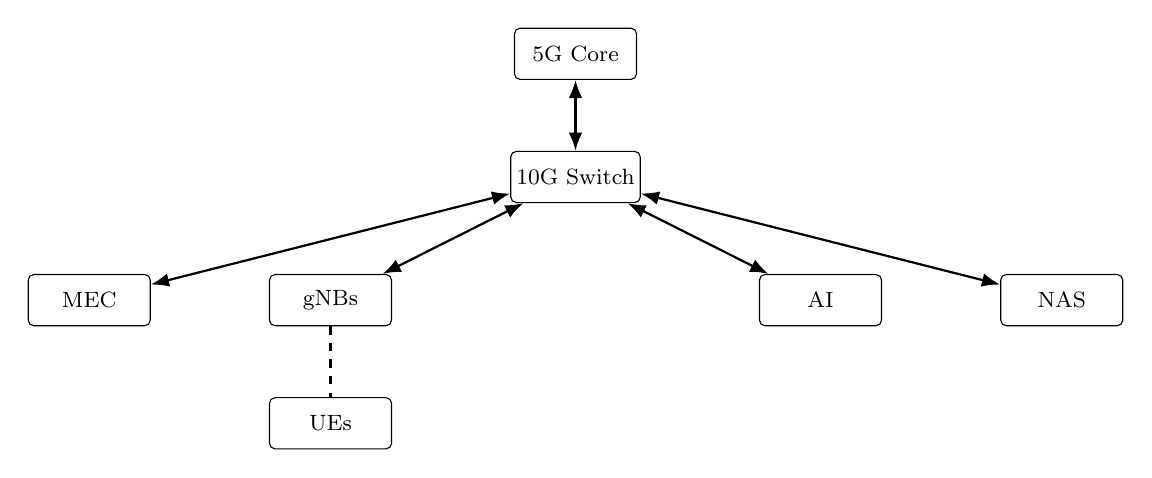
\begin{tikzpicture}[
		>=Latex,
		every node/.style={
			draw,
			rounded corners=2pt,
			minimum width=1.55cm,
			minimum height=0.65cm,
			inner sep=2pt,
			align=center,
			font=\footnotesize
		}
		]
		
		%--------------------------------------------------
		% Nodes
		%--------------------------------------------------
		
		\node (core) {5G Core};
		
		\node (switch) [below=0.9cm of core]
		{10G Switch};
		
		\node (ran) [below left=0.9cm and 1.5cm of switch]
		{gNBs};
		
		\node (ai) [below right=0.9cm and 1.5cm of switch]
		{AI};
		
		\node (mec) [left=1.5cm of ran]
		{MEC};
		
		\node (nas) [right=1.5cm of ai]
		{NAS};
		
		\node (ue) [below=0.9cm of ran]
		{UEs};
		
		%--------------------------------------------------
		% Connections
		%--------------------------------------------------
		
		\draw[<->,thick] (core) -- (switch);
		
		\draw[<->,thick] (switch) -- (ran);
		
		\draw[<->,thick] (switch) -- (ai);
		
		\draw[<->,thick] (switch) -- (mec);
		
		\draw[<->,thick] (switch) -- (nas);
		
		\draw[dashed,thick] (ran) -- (ue);
		
	\end{tikzpicture}
	
	\caption{Interaction Between Major Hardware Components.}
	\label{fig:hardware_interaction}
	
\end{figure}
	
	%%%%%%%%%%%%%%%%%%%%%%%%%%%%%%%%%%%%%%%%%%%%%%%%%%%%%%%%%%%%%%%%%%%%%%%%%%%%%%%
	
	\subsection{Scalability Considerations}
	
	The proposed hardware architecture is intentionally modular and supports incremental expansion.
	
	Future upgrades may include
	
	\begin{itemize}
		
		\item Four or more gNodeBs
		
		\item Additional UPFs
		
		\item Distributed MEC clusters
		
		\item O-RAN Near-RT RIC
		
		\item Massive MIMO radios
		
		\item AI-native orchestration platforms
		
		\item 6G research extensions
		
	\end{itemize}
	
	The modular architecture ensures that future hardware additions can be incorporated without requiring significant redesign of the existing infrastructure.
	
	\section{Proposed Testbed Architecture}
	
	The proposed testbed is designed as a multi-tier private 5G network. It features standard 3GPP control interfaces alongside custom interfaces for AI control and telemetry collection.
	
	\subsection{Logical Architecture} illustrates the logical layout of the testbed, highlighting the interaction between the User Equipments, the SDR-based gNodeBs, the Open5GS Core Network, the MEC servers, and the AI Mobility Controller.
	
	\begin{figure}[htbp]
		\centering
		
		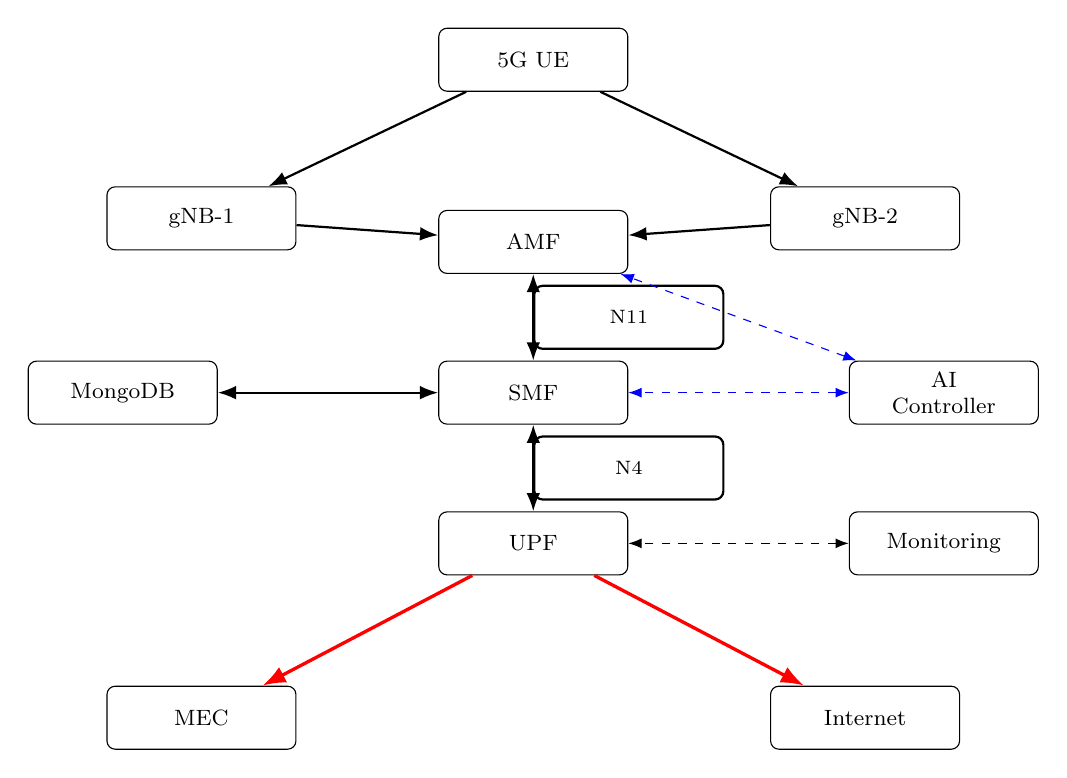
\begin{tikzpicture}[
			>=Latex,
			every node/.style={
				draw,
				rounded corners=3pt,
				minimum width=2.4cm,
				minimum height=0.8cm,
				align=center,
				font=\footnotesize
			}
			]
			
			%%%%%%%%%%%%%%%%%%%%%%%%%%%%%%%%%%%%%%%%%%%%%%%%%%%%%%%%%%%%
			% Top Layer
			%%%%%%%%%%%%%%%%%%%%%%%%%%%%%%%%%%%%%%%%%%%%%%%%%%%%%%%%%%%%
			
			\node (ue) {5G UE};
			
			%%%%%%%%%%%%%%%%%%%%%%%%%%%%%%%%%%%%%%%%%%%%%%%%%%%%%%%%%%%%
			% RAN Layer
			%%%%%%%%%%%%%%%%%%%%%%%%%%%%%%%%%%%%%%%%%%%%%%%%%%%%%%%%%%%%
			
			\node (gnb1) [below left=1.2cm and 1.8cm of ue]
			{gNB-1};
			
			\node (gnb2) [below right=1.2cm and 1.8cm of ue]
			{gNB-2};
			
			%%%%%%%%%%%%%%%%%%%%%%%%%%%%%%%%%%%%%%%%%%%%%%%%%%%%%%%%%%%%
			% Core Layer
			%%%%%%%%%%%%%%%%%%%%%%%%%%%%%%%%%%%%%%%%%%%%%%%%%%%%%%%%%%%%
			
			\node (amf) [below=1.5cm of ue]
			{AMF};
			
			\node (smf) [below=1.1cm of amf]
			{SMF};
			
			\node (upf) [below=1.1cm of smf]
			{UPF};
			
			%%%%%%%%%%%%%%%%%%%%%%%%%%%%%%%%%%%%%%%%%%%%%%%%%%%%%%%%%%%%
			% Bottom Layer
			%%%%%%%%%%%%%%%%%%%%%%%%%%%%%%%%%%%%%%%%%%%%%%%%%%%%%%%%%%%%
			
			\node (mec) [below left=1.4cm and 1.8cm of upf]
			{MEC};
			
			\node (internet) [below right=1.4cm and 1.8cm of upf]
			{Internet};
			
			%%%%%%%%%%%%%%%%%%%%%%%%%%%%%%%%%%%%%%%%%%%%%%%%%%%%%%%%%%%%
			% Side Components
			%%%%%%%%%%%%%%%%%%%%%%%%%%%%%%%%%%%%%%%%%%%%%%%%%%%%%%%%%%%%
			
			\node (mongo) [left=2.8cm of smf]
			{MongoDB};
			
			\node (ai) [right=2.8cm of smf]
			{AI\\Controller};
			
			\node (monitor) [right=2.8cm of upf]
			{Monitoring};
			
			%%%%%%%%%%%%%%%%%%%%%%%%%%%%%%%%%%%%%%%%%%%%%%%%%%%%%%%%%%%%
			% Connections
			%%%%%%%%%%%%%%%%%%%%%%%%%%%%%%%%%%%%%%%%%%%%%%%%%%%%%%%%%%%%
			
			% UE to RAN
			
			\draw[->,thick] (ue) -- (gnb1);
			
			\draw[->,thick] (ue) -- (gnb2);
			
			% RAN to Core
			
			\draw[->,thick] (gnb1) -- (amf);
			
			\draw[->,thick] (gnb2) -- (amf);
			
			% Core
			
			\draw[<->,thick] (amf) -- node[right,font=\scriptsize]{N11} (smf);
			
			\draw[<->,thick] (smf) -- node[right,font=\scriptsize]{N4} (upf);
			
			% User Plane
			
			\draw[->,very thick,red] (upf) -- (mec);
			
			\draw[->,very thick,red] (upf) -- (internet);
			
			% Database
			
			\draw[<->,thick] (mongo) -- (smf);
			
			% AI
			
			\draw[<->,dashed,blue] (ai) -- (amf);
			
			\draw[<->,dashed,blue] (ai) -- (smf);
			
			% Monitoring
			
			\draw[<->,dashed] (monitor) -- (upf);
			
			%%%%%%%%%%%%%%%%%%%%%%%%%%%%%%%%%%%%%%%%%%%%%%%%%%%%%%%%%%%%
			
		\end{tikzpicture}
		
		\caption{Logical Architecture of the Proposed AI-Assisted 5G Mobility Testbed.}
		
		\label{fig:logical_architecture}
		
	\end{figure}
	
	\subsection{End-to-End UE Registration Flow}
	
	\subsection{Physical Deployment Topology} shows the physical deployment topology, illustrating how the hardware modules are interconnected using a Managed L2/L3 switch. All servers, workstations, and storage arrays are connected via high-speed Ethernet (1G/10G) to minimize control-plane latency.
	
	\begin{figure}[htbp]
		\centering
		
		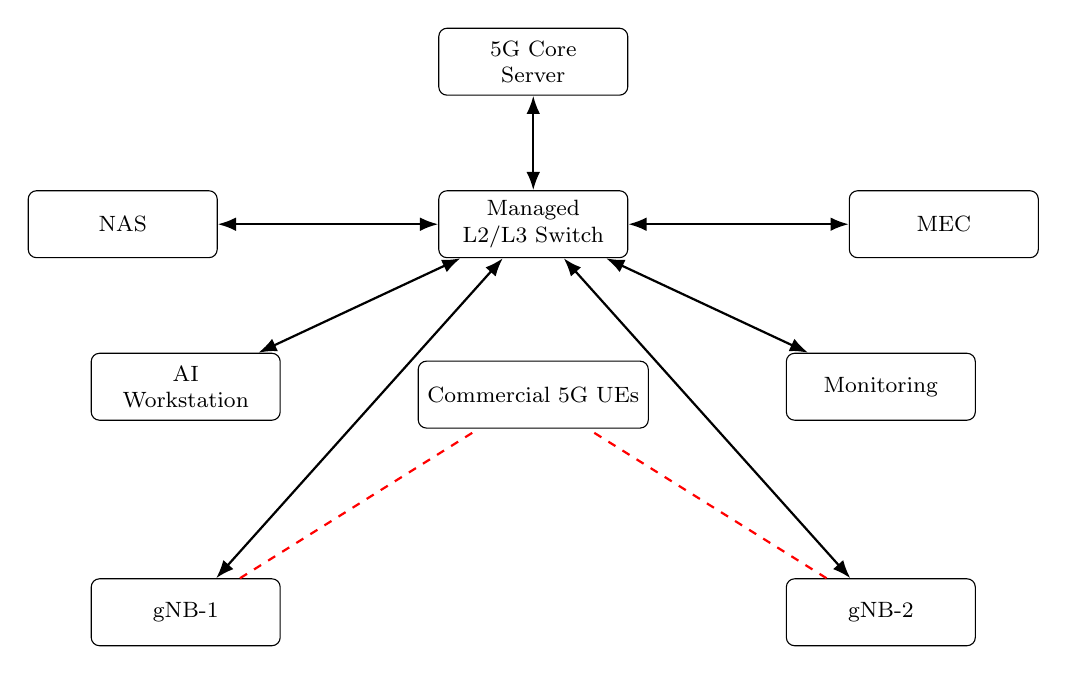
\begin{tikzpicture}[
			>=Latex,
			every node/.style={
				draw,
				rounded corners=3pt,
				minimum width=2.4cm,
				minimum height=0.85cm,
				align=center,
				font=\footnotesize
			}
			]
			
			%%%%%%%%%%%%%%%%%%%%%%%%%%%%%%%%%%%%%%%%%%%%%%%%%%%%%%%%%%%%
			% Core Infrastructure
			%%%%%%%%%%%%%%%%%%%%%%%%%%%%%%%%%%%%%%%%%%%%%%%%%%%%%%%%%%%%
			
			\node (core) {5G Core\\Server};
			
			\node (switch) [below=1.2cm of core]
			{Managed\\L2/L3 Switch};
			
			%%%%%%%%%%%%%%%%%%%%%%%%%%%%%%%%%%%%%%%%%%%%%%%%%%%%%%%%%%%%
			% Compute Layer
			%%%%%%%%%%%%%%%%%%%%%%%%%%%%%%%%%%%%%%%%%%%%%%%%%%%%%%%%%%%%
			
			\node (nas) [left=2.8cm of switch]
			{NAS};
			
			\node (mec) [right=2.8cm of switch]
			{MEC};
			
			\node (ai) [below left=1.2cm and 2.0cm of switch]
			{AI\\Workstation};
			
			\node (monitor) [below right=1.2cm and 2.0cm of switch]
			{Monitoring};
			
			%%%%%%%%%%%%%%%%%%%%%%%%%%%%%%%%%%%%%%%%%%%%%%%%%%%%%%%%%%%%
			% Radio Layer
			%%%%%%%%%%%%%%%%%%%%%%%%%%%%%%%%%%%%%%%%%%%%%%%%%%%%%%%%%%%%
			
			\node (gnb1) [below=2.0cm of ai]
			{gNB-1};
			
			\node (gnb2) [below=2.0cm of monitor]
			{gNB-2};
			
			%%%%%%%%%%%%%%%%%%%%%%%%%%%%%%%%%%%%%%%%%%%%%%%%%%%%%%%%%%%%
			% User Equipment
			%%%%%%%%%%%%%%%%%%%%%%%%%%%%%%%%%%%%%%%%%%%%%%%%%%%%%%%%%%%%
			
			\node (ue) [below=1.3cm of switch]
			{Commercial 5G UEs};
			
			%%%%%%%%%%%%%%%%%%%%%%%%%%%%%%%%%%%%%%%%%%%%%%%%%%%%%%%%%%%%
			% Connections
			%%%%%%%%%%%%%%%%%%%%%%%%%%%%%%%%%%%%%%%%%%%%%%%%%%%%%%%%%%%%
			
			% Core
			
			\draw[<->,thick] (core) -- (switch);
			
			% Infrastructure
			
			\draw[<->,thick] (switch) -- (nas);
			
			\draw[<->,thick] (switch) -- (mec);
			
			\draw[<->,thick] (switch) -- (ai);
			
			\draw[<->,thick] (switch) -- (monitor);
			
			% SDR
			
			\draw[<->,thick] (switch) -- (gnb1);
			
			\draw[<->,thick] (switch) -- (gnb2);
			
			% RF
			
			\draw[dashed,red,thick]
			(gnb1) -- (ue);
			
			\draw[dashed,red,thick]
			(gnb2) -- (ue);
			
		\end{tikzpicture}
		
		\caption{Physical Hardware Deployment Topology.}
		
		\label{fig:physical_architecture}
		
	\end{figure}
	
	%%%%%%%%%%%%%%%%%%%%%%%%%%%%%%%%%%%%%%%%%%%%%%%%%%%%%%%%%%%%%%%%%%%%%%%%%%%%%%%%%%
	\section{System Design and End-to-End Operational Architecture}
	
	The proposed testbed has been designed as a layered cyber-physical system that integrates radio access, core networking, edge computing, artificial intelligence, monitoring, and storage into a unified experimental platform. Unlike conventional laboratory deployments where individual subsystems operate independently, the proposed architecture enables continuous information exchange across every layer of the communication stack.
	
	The complete system follows a closed-loop architecture in which network measurements continuously influence mobility decisions, resource allocation, network slice selection, and edge service placement.
	
	%%%%%%%%%%%%%%%%%%%%%%%%%%%%%%%%%%%%%%%%%%%%%%%%%%%%%%%%%%%%%%%%%%%%%%%%%%%%%%%
	
	\subsection{Layered System Architecture}
	
	The proposed testbed is organized into seven logical layers.
	
	\begin{figure}[h]
		
		\centering
		
		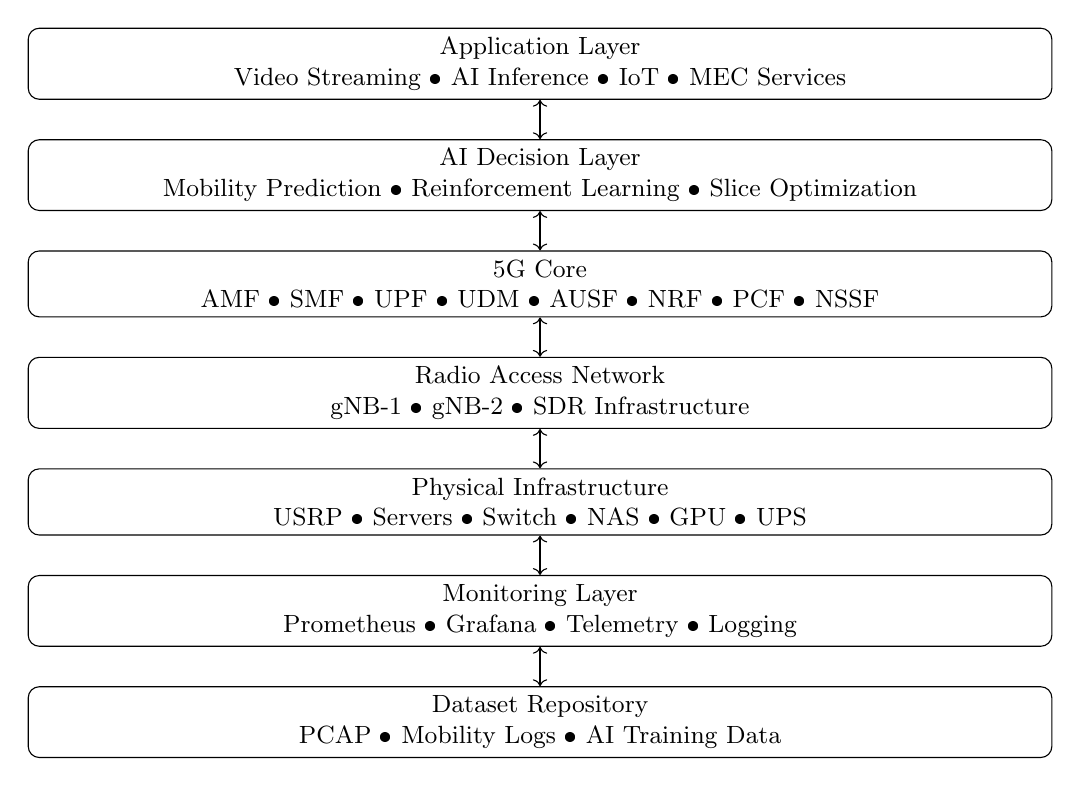
\begin{tikzpicture}[every node/.style={
				draw,
				minimum width=13cm,
				minimum height=0.8cm,
				align=center,
				rounded corners,
				font=\small
			},
			node distance=0.5cm]
			
			\node(app){Application Layer\\Video Streaming • AI Inference • IoT • MEC Services};
			
			\node(ai)[below=of app]{AI Decision Layer\\Mobility Prediction • Reinforcement Learning • Slice Optimization};
			
			\node(core)[below=of ai]{5G Core\\AMF • SMF • UPF • UDM • AUSF • NRF • PCF • NSSF};
			
			\node(ran)[below=of core]{Radio Access Network\\gNB-1 • gNB-2 • SDR Infrastructure};
			
			\node(hw)[below=of ran]{Physical Infrastructure\\USRP • Servers • Switch • NAS • GPU • UPS};
			
			\node(mon)[below=of hw]{Monitoring Layer\\Prometheus • Grafana • Telemetry • Logging};
			
			\node(storage)[below=of mon]{Dataset Repository\\PCAP • Mobility Logs • AI Training Data};
			
			\draw[<->](app)--(ai);
			
			\draw[<->](ai)--(core);
			
			\draw[<->](core)--(ran);
			
			\draw[<->](ran)--(hw);
			
			\draw[<->](hw)--(mon);
			
			\draw[<->](mon)--(storage);
			
		\end{tikzpicture}
		
		\caption{Layered Architecture of the Proposed Research Testbed}
		
		\label{fig:layered_architecture}
		
	\end{figure}
	
	%%%%%%%%%%%%%%%%%%%%%%%%%%%%%%%%%%%%%%%%%%%%%%%%%%%%%%%%%%%%%%%%%%%%%%%%%%%%%%%
	
	\subsection{Operational Workflow}
	
	The complete operation of the proposed system follows eight sequential stages.
	
	\begin{enumerate}
		
		\item User Equipment powers on.
		
		\item UE registers with the nearest gNodeB.
		
		\item Authentication is completed by the 5G Core.
		
		\item A PDU Session is established.
		
		\item AI Mobility Controller begins collecting telemetry.
		
		\item User starts moving across multiple cells.
		
		\item AI predicts future mobility and prepares neighboring cells.
		
		\item Handover completes with uninterrupted IP connectivity.
		
	\end{enumerate}
	
	%%%%%%%%%%%%%%%%%%%%%%%%%%%%%%%%%%%%%%%%%%%%%%%%%%%%%%%%%%%%%%%%%%%%%%%%%%%%%%%
	
	\subsection{Closed-Loop System Operation}
	
	Unlike conventional cellular deployments that react to radio degradation, the proposed architecture continuously monitors the entire network.
	
	The operational feedback loop consists of
	
	\begin{figure}[htbp]
		\centering
		
		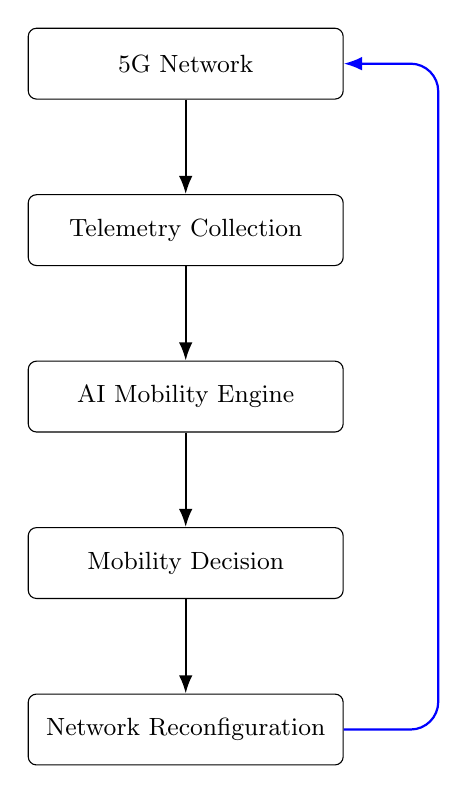
\begin{tikzpicture}[
			>=Latex,
			every node/.style={
				draw,
				rounded corners=3pt,
				minimum width=4.0cm,
				minimum height=0.9cm,
				align=center,
				font=\small
			}
			]
			
			%%%%%%%%%%%%%%%%%%%%%%%%%%%%%%%%%%%%%%%%%%%%%%%%%%%%%%
			% Nodes
			%%%%%%%%%%%%%%%%%%%%%%%%%%%%%%%%%%%%%%%%%%%%%%%%%%%%%%
			
			\node (network) {5G Network};
			
			\node (telemetry) [below=1.2cm of network]
			{Telemetry Collection};
			
			\node (ai) [below=1.2cm of telemetry]
			{AI Mobility Engine};
			
			\node (decision) [below=1.2cm of ai]
			{Mobility Decision};
			
			\node (execute) [below=1.2cm of decision]
			{Network Reconfiguration};
			
			%%%%%%%%%%%%%%%%%%%%%%%%%%%%%%%%%%%%%%%%%%%%%%%%%%%%%%
			% Forward Flow
			%%%%%%%%%%%%%%%%%%%%%%%%%%%%%%%%%%%%%%%%%%%%%%%%%%%%%%
			
			\draw[->,thick]
			(network) -- (telemetry);
			
			\draw[->,thick]
			(telemetry) -- (ai);
			
			\draw[->,thick]
			(ai) -- (decision);
			
			\draw[->,thick]
			(decision) -- (execute);
			
			%%%%%%%%%%%%%%%%%%%%%%%%%%%%%%%%%%%%%%%%%%%%%%%%%%%%%%
			% Feedback Loop
			%%%%%%%%%%%%%%%%%%%%%%%%%%%%%%%%%%%%%%%%%%%%%%%%%%%%%%
			
			\draw[
			->,
			thick,
			blue,
			rounded corners=10pt
			]
			(execute.east)
			-- ++(1.2,0)
			|- 
			(network.east);
			
			%%%%%%%%%%%%%%%%%%%%%%%%%%%%%%%%%%%%%%%%%%%%%%%%%%%%%%
			
		\end{tikzpicture}
		
		\caption{Closed-Loop AI-Assisted Mobility Optimization Framework.}
		
		\label{fig:closed_loop_system}
		
	\end{figure}
	
	%%%%%%%%%%%%%%%%%%%%%%%%%%%%%%%%%%%%%%%%%%%%%%%%%%%%%%%%%%%%%%%%%%%%%%%%%%%%%%%
	
	\subsection{End-to-End Data Flow}
	
	 illustrates the complete path followed by signaling messages and user traffic throughout the proposed infrastructure.
	
	\begin{figure}[htbp]
		\centering
		
		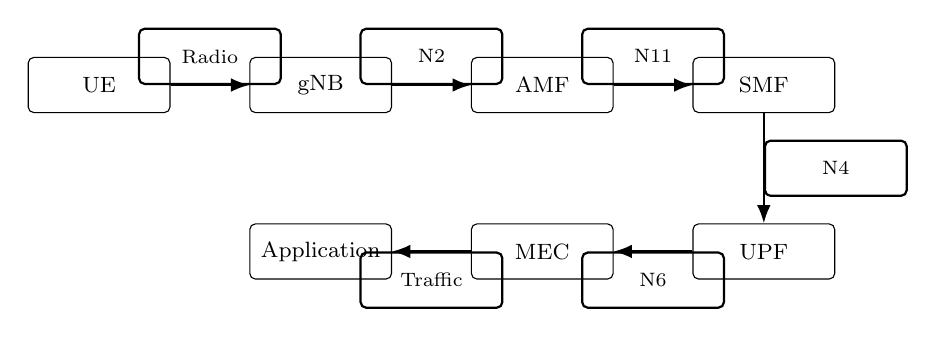
\begin{tikzpicture}[
			>=Latex,
			every node/.style={
				draw,
				rounded corners=2pt,
				minimum width=1.8cm,
				minimum height=0.7cm,
				font=\footnotesize,
				align=center
			}
			]
			
			%--------------------------------------------------
			% Top Row
			%--------------------------------------------------
			
			\node (ue) {UE};
			
			\node (gnb) [right=1.0cm of ue] {gNB};
			
			\node (amf) [right=1.0cm of gnb] {AMF};
			
			\node (smf) [right=1.0cm of amf] {SMF};
			
			%--------------------------------------------------
			% Bottom Row
			%--------------------------------------------------
			
			\node (upf) [below=1.4cm of smf] {UPF};
			
			\node (mec) [left=1.0cm of upf] {MEC};
			
			\node (app) [left=1.0cm of mec] {Application};
			
			%--------------------------------------------------
			% Flow
			%--------------------------------------------------
			
			\draw[->,thick]
			(ue) -- node[above,font=\scriptsize]{Radio} (gnb);
			
			\draw[->,thick]
			(gnb) -- node[above,font=\scriptsize]{N2} (amf);
			
			\draw[->,thick]
			(amf) -- node[above,font=\scriptsize]{N11} (smf);
			
			\draw[->,thick]
			(smf) -- node[right,font=\scriptsize]{N4} (upf);
			
			\draw[->,thick]
			(upf) -- node[below,font=\scriptsize]{N6} (mec);
			
			\draw[->,thick]
			(mec) -- node[below,font=\scriptsize]{Traffic} (app);
			
		\end{tikzpicture}
		
		\caption{End-to-End Operational Data Flow.}
		\label{fig:dataflow_complete}
		
	\end{figure}
	
	%%%%%%%%%%%%%%%%%%%%%%%%%%%%%%%%%%%%%%%%%%%%%%%%%%%%%%%%%%%%%%%%%%%%%%%%%%%%%%%
	
	\subsection{Component Interaction Matrix}
	
	Table~\ref{tab} summarizes the interaction between the major hardware and software components.
	
	\begin{table}[h]
		
		\centering
		
		\caption{Major Component Interactions}
		
		\label{tab:interaction}
		
		\begin{tabular}{lll}
			
			\toprule
			
			Source
			
			&
			
			Destination
			
			&
			
			Purpose
			
			\\
			
			\midrule
			
			UE & gNB & Radio Access
			
			\\
			
			gNB & AMF & Registration
			
			\\
			
			AMF & UDM & Authentication
			
			\\
			
			AMF & SMF & Session Management
			
			\\
			
			SMF & UPF & Tunnel Creation
			
			\\
			
			UPF & MEC & Edge Traffic
			
			\\
			
			UPF & Internet & External Access
			
			\\
			
			Prometheus & AI & Telemetry
			
			\\
			
			AI & AMF & Mobility Decision
			
			\\
			
			AI & SMF & Slice Decision
			
			\\
			
			AI & MEC & Service Migration
			
			\\
			
			Grafana & Operators & Monitoring
			
			\\
			
			\bottomrule
			
		\end{tabular}
		
	\end{table}
	
	%%%%%%%%%%%%%%%%%%%%%%%%%%%%%%%%%%%%%%%%%%%%%%%%%%%%%%%%%%%%%%%%%%%%%%%%%%%%%%%
	
	\subsection{Data Lifecycle}
	
	Every experiment conducted on the proposed platform generates multiple forms of telemetry.
	
	The lifecycle of experimental data consists of
	
	\begin{enumerate}
		
		\item Packet Capture
		
		\item KPI Collection
		
		\item Time Synchronization
		
		\item Storage
		
		\item Dataset Construction
		
		\item AI Training
		
		\item Evaluation
		
		\item Publication
		
	\end{enumerate}
	
	This standardized pipeline ensures reproducibility of all experimental results and enables long-term dataset creation for future machine learning research.
	
	%%%%%%%%%%%%%%%%%%%%%%%%%%%%%%%%%%%%%%%%%%%%%%%%%%%%%%%%%%%%%%%%%%%%%%%%%%%%%%%
	
	\subsection{System Design Advantages}
	
	Compared to existing software-only simulators, the proposed architecture provides
	
	\begin{itemize}
		
		\item Real radio propagation
		
		\item Physical SDR hardware
		
		\item Commercial User Equipments
		
		\item Standards-compliant 5G Core
		
		\item Edge Computing
		
		\item AI-assisted Mobility
		
		\item Network Slice Orchestration
		
		\item Continuous Telemetry
		
		\item Real-time Dataset Generation
		
		\item Future Open RAN compatibility
		
		\item Expandability toward AI-native 6G
		
	\end{itemize}
	
	Consequently, the proposed infrastructure serves as a complete experimental ecosystem capable of supporting both current 5G research and future Beyond-5G investigations.
	
	\newpage
	
	%%%%%%%%%%%%%%%%%%%%%%%%%%%%%%%%%%%%%%%%%%%%%%%%%%%%%%%%%%%%%%%%%%%%%%%%%%%%%%%%%%
	\section{Technical Justification of the Proposed Infrastructure}
	
	The successful realization of a realistic 5G Standalone research testbed requires considerably more than the deployment of a software-based core network and a pair of Software Defined Radios (SDRs). A complete experimental platform must reproduce the behaviour of commercial cellular infrastructure while providing sufficient flexibility to modify network functions, evaluate mobility algorithms, collect telemetry, and perform large-scale Artificial Intelligence (AI) experimentation.
	
	Each hardware subsystem proposed in this project has therefore been selected based on its functional necessity rather than merely its computational capability. The following subsections justify the inclusion of every major infrastructure component within the proposed laboratory.
	
	%%%%%%%%%%%%%%%%%%%%%%%%%%%%%%%%%%%%%%%%%%%%%%%%%%%%%%%%%%%%%%%%%%%%%%%%%%%%%%%
	
	\subsection{5G Core Server}
	
	The Core Server forms the central control entity of the private cellular network. It simultaneously hosts multiple Network Functions including the Access and Mobility Management Function (AMF), Session Management Function (SMF), User Plane Function (UPF), Unified Data Management (UDM), Authentication Server Function (AUSF), Policy Control Function (PCF), Network Repository Function (NRF), and Network Slice Selection Function (NSSF).
	
	A high-performance rack-mounted server is required because these services execute concurrently while processing large volumes of signaling traffic and user-plane packets. The use of enterprise-grade processors and high-speed storage minimizes processing latency during mobility procedures and ensures reliable long-duration operation.
	
	%%%%%%%%%%%%%%%%%%%%%%%%%%%%%%%%%%%%%%%%%%%%%%%%%%%%%%%%%%%%%%%%%%%%%%%%%%%%%%%
	
	\subsection{Software Defined Radios}
	
	Unlike traditional networking experiments, mobility research requires actual radio transmission and reception. Software Defined Radios replace proprietary base station hardware and provide complete access to the physical layer.
	
	The selected Ettus USRP B210 platform enables implementation of programmable gNodeBs supporting realistic radio transmission, scheduling, and mobility procedures. Two independent SDR platforms are required to establish overlapping radio cells and facilitate inter-cell handover experiments.
	
	%%%%%%%%%%%%%%%%%%%%%%%%%%%%%%%%%%%%%%%%%%%%%%%%%%%%%%%%%%%%%%%%%%%%%%%%%%%%%%%
	
	\subsection{Commercial User Equipments}
	
	Software-based User Equipment simulators cannot accurately reproduce the radio characteristics, hardware timing, modem behaviour, and protocol implementations found in commercial devices.
	
	Accordingly, the proposed laboratory employs commercial 5G smartphones operating in Standalone (SA) mode. These devices execute complete 3GPP procedures including registration, authentication, PDU session establishment, mobility management, and application-layer traffic generation.
	
	%%%%%%%%%%%%%%%%%%%%%%%%%%%%%%%%%%%%%%%%%%%%%%%%%%%%%%%%%%%%%%%%%%%%%%%%%%%%%%%
	
	\subsection{Multi-access Edge Computing Server}
	
	Emerging 5G applications increasingly rely upon edge computing to reduce application latency. During user mobility, application services may require migration between edge servers while preserving session continuity.
	
	A dedicated MEC server therefore enables investigation of edge-aware mobility management, service migration, traffic steering, and intelligent workload placement.
	
	%%%%%%%%%%%%%%%%%%%%%%%%%%%%%%%%%%%%%%%%%%%%%%%%%%%%%%%%%%%%%%%%%%%%%%%%%%%%%%%
	
	\subsection{Artificial Intelligence Workstation}
	
	The proposed research incorporates Deep Learning and Reinforcement Learning models that continuously analyse network telemetry and predict future mobility events.
	
	Training these models requires substantial computational resources including GPU acceleration, high-bandwidth memory, and fast storage. The AI workstation therefore performs both offline model training and online inference during experimental evaluation.
	
	%%%%%%%%%%%%%%%%%%%%%%%%%%%%%%%%%%%%%%%%%%%%%%%%%%%%%%%%%%%%%%%%%%%%%%%%%%%%%%%
	
	\subsection{Monitoring Server}
	
	Objective evaluation of mobility algorithms requires continuous monitoring of every subsystem within the laboratory.
	
	The monitoring server aggregates telemetry collected from the 5G Core, SDR hosts, User Equipments, AI controller, MEC server, and networking infrastructure. Prometheus exporters periodically collect system metrics, while Grafana dashboards provide real-time visualization of network behaviour throughout each experiment.
	
	%%%%%%%%%%%%%%%%%%%%%%%%%%%%%%%%%%%%%%%%%%%%%%%%%%%%%%%%%%%%%%%%%%%%%%%%%%%%%%%
	
	\subsection{Network Attached Storage}
	
	Every mobility experiment generates significant volumes of packet captures, telemetry logs, application traces, and machine learning datasets.
	
	A dedicated Network Attached Storage (NAS) appliance provides centralized, fault-tolerant storage for long-term archival and enables multiple researchers to access experimental datasets simultaneously without impacting operational servers.
	
	%%%%%%%%%%%%%%%%%%%%%%%%%%%%%%%%%%%%%%%%%%%%%%%%%%%%%%%%%%%%%%%%%%%%%%%%%%%%%%%
	
	\subsection{Networking Infrastructure}
	
	The networking subsystem interconnects all compute nodes through a managed Layer-2/Layer-3 Ethernet switch supporting Gigabit and 10 Gigabit communication.
	
	High-bandwidth switching minimizes packet forwarding latency between the Core Network, MEC server, AI workstation, and monitoring infrastructure. It additionally supports VLAN segmentation for isolating control-plane, user-plane, management, and storage traffic.
	
	%%%%%%%%%%%%%%%%%%%%%%%%%%%%%%%%%%%%%%%%%%%%%%%%%%%%%%%%%%%%%%%%%%%%%%%%%%%%%%%
	
	\subsection{Power Infrastructure}
	
	Research experiments frequently execute continuously for several hours or even days. Unexpected power interruptions may invalidate experimental results and damage sensitive equipment.
	
	The proposed Online UPS system provides uninterrupted electrical power, surge protection, and controlled shutdown capability during extended power failures, thereby preserving both experimental data and hardware reliability.
	
	%%%%%%%%%%%%%%%%%%%%%%%%%%%%%%%%%%%%%%%%%%%%%%%%%%%%%%%%%%%%%%%%%%%%%%%%%%%%%%%
	
	\subsection{Infrastructure Integration}
	
	The proposed infrastructure has been designed according to three fundamental engineering principles:
	
	\begin{enumerate}
		
		\item \textbf{Functional Isolation}
		
		Critical services such as the 5G Core, AI controller, MEC applications, monitoring platform, and storage infrastructure execute on dedicated hardware, eliminating resource contention.
		
		\item \textbf{Modular Expansion}
		
		Every subsystem communicates through standardized interfaces, allowing additional SDRs, MEC servers, User Equipments, and AI accelerators to be integrated without architectural redesign.
		
		\item \textbf{Research Flexibility}
		
		The use of programmable Software Defined Radios, open-source 5G software stacks, and containerized deployment enables rapid implementation of new mobility algorithms, network slicing techniques, and future Beyond-5G enhancements.
		
	\end{enumerate}
	
	%%%%%%%%%%%%%%%%%%%%%%%%%%%%%%%%%%%%%%%%%%%%%%%%%%%%%%%%%%%%%%%%%%%%%%%%%%%%%%%
	
	\subsection{Overall Engineering Rationale}
	
	The selected infrastructure represents a balanced compromise between research capability, deployment complexity, and financial feasibility. Each subsystem directly supports one or more research objectives related to intelligent mobility management, AI-assisted handover optimization, network slicing, or edge computing.
	
	Consequently, the proposed laboratory constitutes a reusable experimental platform capable of supporting multiple future research projects beyond the scope of the present proposal, including Open RAN, AI-native networking, Network Digital Twins, and sixth-generation (6G) communication systems.
	
	%%%%%%%%%%%%%%%%%%%%%%%%%%%%%%%%%%%%%%%%%%%%%%%%%%%%%%%%%%%%%%%%%%%%%%%%%%%%%%%%%%
	\section{Deployment Strategy and System Integration}
	
	Following procurement, the proposed testbed will be deployed in a phased manner to ensure incremental validation of every subsystem before full-scale experimental evaluation. Each deployment phase concludes with functional verification to isolate hardware, software, and networking issues before progressing to the next stage.
	
	The deployment strategy minimizes integration risks while providing measurable milestones throughout laboratory establishment.
	
	%%%%%%%%%%%%%%%%%%%%%%%%%%%%%%%%%%%%%%%%%%%%%%%%%%%%%%%%%%%%%%%%%%%%%%%%%%%%%%%
	
	\subsection{Phase I: Laboratory Preparation}
	
	Prior to hardware installation, the laboratory environment will be prepared to accommodate server infrastructure, networking equipment, and radio access hardware.
	
	Activities include
	
	\begin{itemize}
		
		\item Installation of equipment rack
		
		\item Electrical wiring
		
		\item Dedicated UPS connection
		
		\item Air conditioning verification
		
		\item Ethernet backbone installation
		
		\item Cable management
		
		\item Internet uplink provisioning
		
	\end{itemize}
	
	%%%%%%%%%%%%%%%%%%%%%%%%%%%%%%%%%%%%%%%%%%%%%%%%%%%%%%%%%%%%%%%%%%%%%%%%%%%%%%%
	
	\subsection{Phase II: Compute Infrastructure Deployment}
	
	The compute layer forms the foundation of the laboratory.
	
	The following systems are installed and verified.
	
	\begin{itemize}
		
		\item Core Network Server
		
		\item MEC Server
		
		\item AI Workstation
		
		\item Monitoring Server
		
		\item NAS Storage
		
	\end{itemize}
	
	Each system undergoes
	
	\begin{itemize}
		
		\item BIOS validation
		
		\item RAID configuration
		
		\item Operating System installation
		
		\item Network configuration
		
		\item SSH connectivity verification
		
		\item Time synchronization
		
	\end{itemize}
	
	%%%%%%%%%%%%%%%%%%%%%%%%%%%%%%%%%%%%%%%%%%%%%%%%%%%%%%%%%%%%%%%%%%%%%%%%%%%%%%%
	
	\subsection{Phase III: Network Infrastructure Deployment}
	
	The networking layer interconnects all compute nodes.
	
	Deployment activities include
	
	\begin{itemize}
		
		\item Managed switch configuration
		
		\item VLAN creation
		
		\item IP address assignment
		
		\item 10 Gigabit uplink configuration
		
		\item Routing verification
		
		\item Firewall configuration
		
	\end{itemize}
	
	%%%%%%%%%%%%%%%%%%%%%%%%%%%%%%%%%%%%%%%%%%%%%%%%%%%%%%%%%%%%%%%%%%%%%%%%%%%%%%%
	
	\subsection{Phase IV: 5G Core Deployment}
	
	The software components of the 5G Core are deployed using containerized services.
	
	The deployment sequence consists of
	
	\begin{enumerate}
		
		\item MongoDB
		
		\item NRF
		
		\item UDM
		
		\item AUSF
		
		\item AMF
		
		\item SMF
		
		\item PCF
		
		\item NSSF
		
		\item UPF
		
	\end{enumerate}
	
	Following deployment, all Service Based Interfaces (SBIs) are verified using health checks and functional tests.
	
	%%%%%%%%%%%%%%%%%%%%%%%%%%%%%%%%%%%%%%%%%%%%%%%%%%%%%%%%%%%%%%%%%%%%%%%%%%%%%%%
	
	\subsection{Phase V: Radio Access Network Deployment}
	
	Each Software Defined Radio is connected to its host workstation.
	
	Deployment includes
	
	\begin{itemize}
		
		\item UHD Driver installation
		
		\item SDR firmware update
		
		\item Clock synchronization
		
		\item RF calibration
		
		\item gNodeB configuration
		
		\item Cell broadcast verification
		
	\end{itemize}
	
	Commercial User Equipments are then attached to the private network for initial registration testing.
	
	%%%%%%%%%%%%%%%%%%%%%%%%%%%%%%%%%%%%%%%%%%%%%%%%%%%%%%%%%%%%%%%%%%%%%%%%%%%%%%%
	
	\subsection{Phase VI: Monitoring and Telemetry Deployment}
	
	Monitoring infrastructure is activated prior to experimental execution.
	
	Telemetry sources include
	
	\begin{itemize}
		
		\item Core Network metrics
		
		\item SDR statistics
		
		\item Operating system statistics
		
		\item GPU utilization
		
		\item MEC resource usage
		
		\item Network bandwidth
		
		\item Packet captures
		
	\end{itemize}
	
	Grafana dashboards are configured to provide real-time visibility into every subsystem.
	
	%%%%%%%%%%%%%%%%%%%%%%%%%%%%%%%%%%%%%%%%%%%%%%%%%%%%%%%%%%%%%%%%%%%%%%%%%%%%%%%
	
	\subsection{Phase VII: AI Framework Deployment}
	
	After successful validation of the baseline network, the Artificial Intelligence framework is introduced.
	
	Deployment activities include
	
	\begin{itemize}
		
		\item Dataset collection
		
		\item Feature extraction
		
		\item Model training
		
		\item Model validation
		
		\item Online inference deployment
		
		\item Closed-loop testing
		
	\end{itemize}
	
	%%%%%%%%%%%%%%%%%%%%%%%%%%%%%%%%%%%%%%%%%%%%%%%%%%%%%%%%%%%%%%%%%%%%%%%%%%%%%%%
	
	\subsection{System Integration Workflow}
	
	 illustrates the complete deployment pipeline.
	
	\begin{figure}[h]
		
		\centering
		
		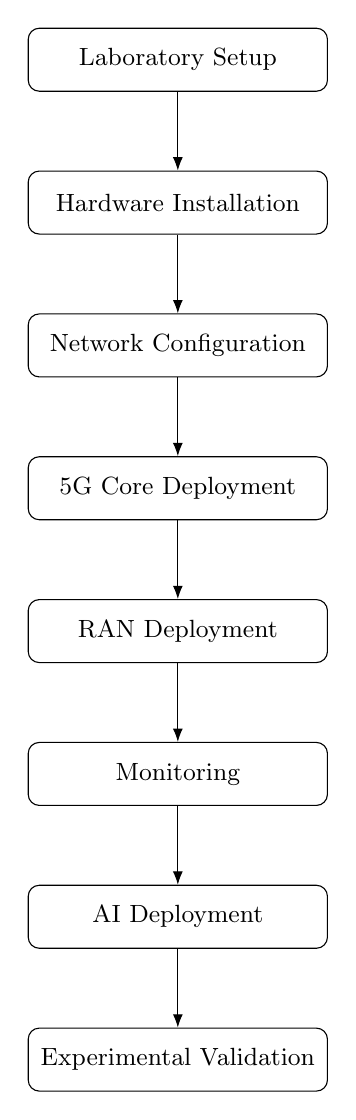
\begin{tikzpicture}[>=Latex,
			node distance=1cm,
			every node/.style={
				draw,
				rounded corners,
				minimum width=3.8cm,
				minimum height=0.8cm,
				align=center,
				font=\small
			}]
			
			\node(lab){Laboratory Setup};
			
			\node(hw)[below=of lab]{Hardware Installation};
			
			\node(net)[below=of hw]{Network Configuration};
			
			\node(core)[below=of net]{5G Core Deployment};
			
			\node(ran)[below=of core]{RAN Deployment};
			
			\node(mon)[below=of ran]{Monitoring};
			
			\node(ai)[below=of mon]{AI Deployment};
			
			\node(exp)[below=of ai]{Experimental Validation};
			
			\draw[->](lab)--(hw);
			
			\draw[->](hw)--(net);
			
			\draw[->](net)--(core);
			
			\draw[->](core)--(ran);
			
			\draw[->](ran)--(mon);
			
			\draw[->](mon)--(ai);
			
			\draw[->](ai)--(exp);
			
		\end{tikzpicture}
		
		\caption{Phased Deployment and Integration Workflow}
		
		\label{fig:deployment_workflow}
		
	\end{figure}
	
	%%%%%%%%%%%%%%%%%%%%%%%%%%%%%%%%%%%%%%%%%%%%%%%%%%%%%%%%%%%%%%%%%%%%%%%%%%%%%%%
	
	\subsection{Verification Checklist}
	
	Each deployment phase concludes with predefined acceptance tests.
	
	\begin{table}[h]
		
		\centering
		
		\caption{Deployment Verification Checklist}
		
		\begin{tabular}{p{6cm}p{5cm}}
			
			\toprule
			
			Subsystem
			
			&
			
			Verification
			
			\\
			
			\midrule
			
			Core Network
			
			&
			
			Successful UE Registration
			
			\\
			
			RAN
			
			&
			
			Cell Broadcast Detection
			
			\\
			
			UPF
			
			&
			
			Internet Connectivity
			
			\\
			
			MEC
			
			&
			
			Application Deployment
			
			\\
			
			AI Controller
			
			&
			
			Real-Time Inference
			
			\\
			
			Monitoring
			
			&
			
			Live Dashboard
			
			\\
			
			NAS
			
			&
			
			Log Archival
			
			\\
			
			Mobility
			
			&
			
			Successful Handover
			
			\\
			
			\bottomrule
			
		\end{tabular}
		
	\end{table}
	
	%%%%%%%%%%%%%%%%%%%%%%%%%%%%%%%%%%%%%%%%%%%%%%%%%%%%%%%%%%%%%%%%%%%%%%%%%%%%%%%
	
	\subsection{Expected Deployment Duration}
	
	The complete infrastructure is expected to be operational within approximately twelve weeks following procurement.
	
	\begin{table}[h]
		
		\centering
		
		\caption{Estimated Deployment Timeline}
		
		\begin{tabular}{lc}
			
			\toprule
			
			Activity
			
			&
			
			Duration
			
			\\
			
			\midrule
			
			Laboratory Preparation
			
			&
			
			2 Weeks
			
			\\
			
			Hardware Installation
			
			&
			
			2 Weeks
			
			\\
			
			Network Configuration
			
			&
			
			1 Week
			
			\\
			
			5G Core Installation
			
			&
			
			2 Weeks
			
			\\
			
			RAN Deployment
			
			&
			
			2 Weeks
			
			\\
			
			AI Integration
			
			&
			
			2 Weeks
			
			\\
			
			System Validation
			
			&
			
			1 Week
			
			\\
			
			\bottomrule
			
		\end{tabular}
		
	\end{table}
	
	\section{Required Modules and Procurement Matrix}
	
	The hardware requirements for the proposed 5G testbed are structured into nine distinct modules. Table provides a detailed procurement matrix outlining the hardware components, specifications, target pricing, and verified vendors in India.
	
\begin{longtable}{
		p{1.7cm}
		p{2cm}
		p{4cm}
		c
		p{2.8cm}
		p{3 cm}
	}
	
	\caption{Procurement and Module Matrix for the Proposed 5G Standalone Testbed}
	\label{tab:procurement_matrix}\\
	
	\toprule
	\textbf{Subsystem} &
	\textbf{Module Details} &
	\textbf{Key Technical Specifications} &
	\textbf{Qty} &
	\textbf{Procurement Source} &
	\textbf{Estimated Cost (INR)} \\
	\midrule
	\endfirsthead
	
	\multicolumn{6}{c}%
	{{\bfseries Table \thetable\ Continued from Previous Page}} \\
	\toprule
	\textbf{Subsystem} &
	\textbf{Module Details} &
	\textbf{Key Technical Specifications} &
	\textbf{Qty} &
	\textbf{Procurement Source} &
	\textbf{Estimated Cost (INR)} \\
	\midrule
	\endhead
	
	\midrule
	\multicolumn{6}{r}{Continued on Next Page} \\
	\endfoot
	
	\bottomrule
	\endlastfoot
	
	%%%%%%%%%%%%%%%%%%%%%%%%%%%%%%%%%%%%%%%%%%%%%%%%%%%%%%%%%%%%%%%%%%%%%%%
	
	\textbf{1. 5G Core} &
	Dell PowerEdge R760 Rack Server &
	Dual Intel Xeon Silver 4410Y, 128 GB DDR5 RAM, 2 $\times$ 480 GB SSD (RAID-1), Dual 10 GbE SFP+ &
	1 &
	Dell India / ServerBasket India &
	3,50,000 \\
	
	\addlinespace
	
	\textbf{2. 5G RAN} &
	Ettus USRP B210 Software Defined Radio &
	70 MHz--6 GHz, 2$\times$2 MIMO, USB 3.0, SMA RF Interface, External Omni-directional Antennas &
	2 &
	GSAS Micro Systems Bangalore / Element14 India &
	5,00,000 \\
	
	\addlinespace
	
	\textbf{3. User Equipment} &
	Commercial Android 5G Smartphones &
	5G Standalone (SA) Support, NR Band n78, Manual PLMN Selection &
	5 &
	Amazon India / Samsung / OnePlus &
	1,50,000 \\
	
	\addlinespace
	
	\textbf{4. MEC Server} &
	HPE ProLiant DL360 Gen11 &
	Intel Xeon Silver, 64 GB DDR5 RAM, 1.92 TB NVMe SSD, Dual 10 GbE NIC &
	1 &
	HPE India Partner / Cyberwala &
	2,50,000 \\
	
	\addlinespace
	
	\textbf{5. AI Workstation} &
	Custom Liquid-Cooled GPU Workstation &
	Intel Core i9-14900K, NVIDIA RTX 4090 (24 GB), 64 GB DDR5, 2 TB Gen4 NVMe SSD &
	1 &
	Volted PC Delhi / PC Kumar Bangalore &
	3,50,000 \\
	
	\addlinespace
	
	\textbf{6. Monitoring Server} &
	Dell PowerEdge R250 &
	Intel Xeon E-2314, 32 GB RAM, Dual 1 TB HDD, Dual Gigabit Ethernet &
	1 &
	Dell India / ServerBasket India &
	80,000 \\
	
	\addlinespace
	
	\textbf{7. NAS Storage} &
	Synology DS1821+ NAS &
	8-Bay NAS with 4 $\times$ 4 TB Seagate IronWolf HDDs configured in RAID-5 &
	1 &
	Computech Store / Vishal Peripherals &
	1,40,000 \\
	
	\addlinespace
	
	\textbf{8. Networking} &
	Managed L2/L3 Enterprise Switch &
	24-Port Gigabit PoE+, 4 $\times$ 10 Gb SFP+ Uplinks, Cat6A Structured Cabling &
	1 &
	Vishal Peripherals / L\&T SuFin &
	60,000 \\
	
	\addlinespace
	
	\textbf{9. Power Infrastructure} &
	APC Smart-UPS RC 5 kVA &
	Online Double Conversion UPS with External Battery Cabinet (Approx. 30 Minutes Backup) &
	1 &
	APC Schneider Electric India / Vertiv India &
	1,20,000 \\
	
	%%%%%%%%%%%%%%%%%%%%%%%%%%%%%%%%%%%%%%%%%%%%%%%%%%%%%%%%%%%%%%%%%%%%%%%
	
	\midrule
	
	\multicolumn{5}{r}{\textbf{Total Estimated Capital Expenditure (CAPEX)}} &
	\textbf{20,00,000} \\
	
	\bottomrule
	
\end{longtable}
		
		\newpage
		
		\section{Detailed Module Technical Specifications \& Visualizations}This section provides technical descriptions and visual references for the key physical hardware modules to be procured for the laboratory.
		
		\subsection{Module 1: Software-Defined Radio (SDR) RAN Transceiver}The Radio Access Network (RAN) is implemented using the Ettus Research USRP B210. This platform is chosen for its native integration with open-source LTE/5G stacks (srsRAN and OpenAirInterface). It operates as a fully flexible gNodeB base station.
		\begin{itemize}
			\item \textbf{Frequency Range:} 70 MHz to 6 GHz (supporting 5G SA FR1 bands, specifically n78).
			\item \textbf{RF Channels:} 2 $\times$ 2 MIMO transceiver offering up to 56 MHz of real-time bandwidth.
			\item \textbf{Interface:} High-speed USB 3.0 connection to the host PC running srsRAN gNB software.\end{itemize} shows the physical Ettus USRP B210 unit in its metal enclosure, with RF cabling and SMA antennas connected on a laboratory workbench.
		
		\begin{figure}[htbp]
			\centering
			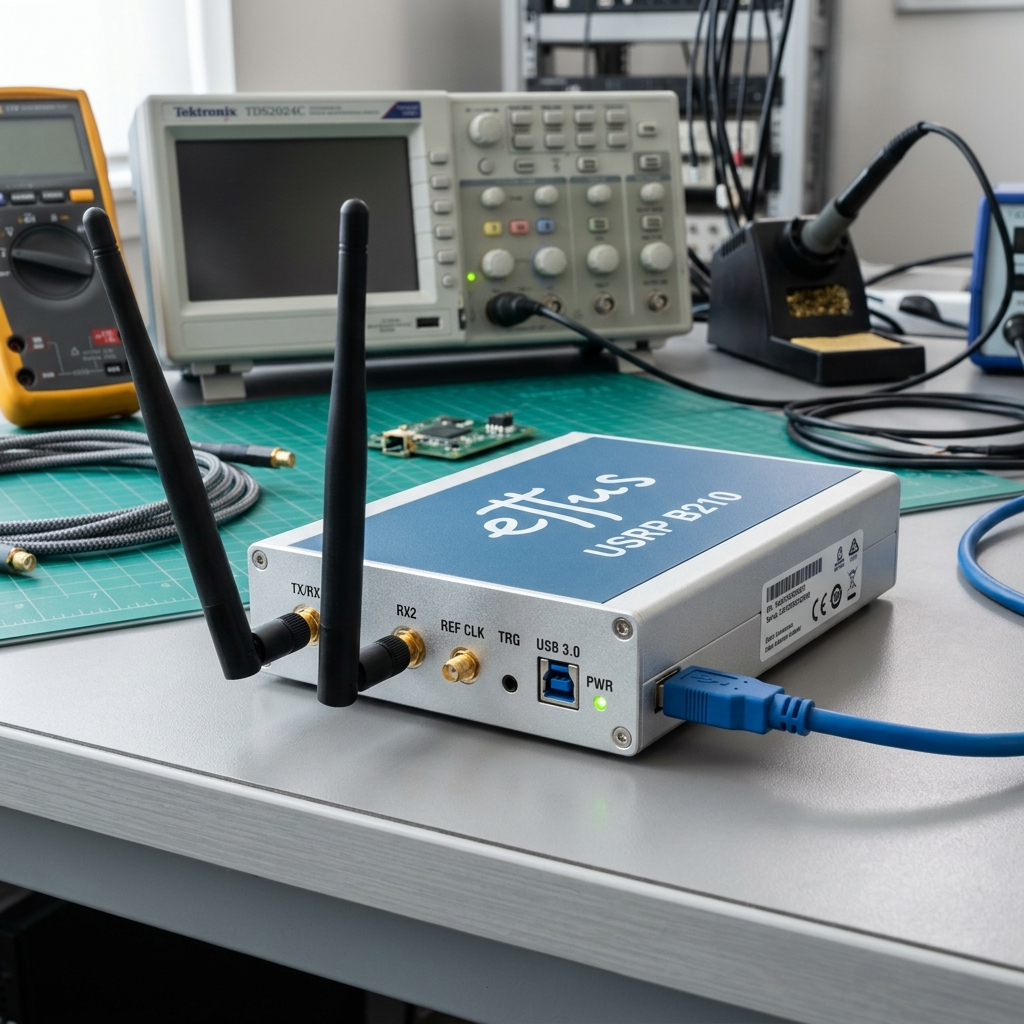
\includegraphics[width=0.6\textwidth]{usrp_b210_sdr.png}
			\caption{Ettus Research USRP B210 SDR Unit (Procured via GSAS Micro Systems)}
			\label{fig}
		\end{figure}
		
		\subsection{Module 2: 5G Core Network Rack Server}The Core Network runs Open5GS. It requires a dedicated, reliable rack-mounted server capable of handling hundreds of subscriber sessions, managing control-plane database queries, and routing high-throughput user-plane traffic (UPF) with low latency.\begin{itemize}\item \textbf{Model:} Dell PowerEdge R760 (2U Rack Server).\item \textbf{Compute:} Dual Intel Xeon Silver processors with hardware virtualization enabled.\item \textbf{Connectivity:} Intel X550 Dual Port 10GbE SFP+ Network Interface Card for low-latency routing to the MEC server and managed switches.\end{itemize} illustrates the front interface of the Dell PowerEdge R760 server showcasing the hot-swappable drive bays and indicator LEDs.
		
		\begin{figure}[htbp]
			\centering
			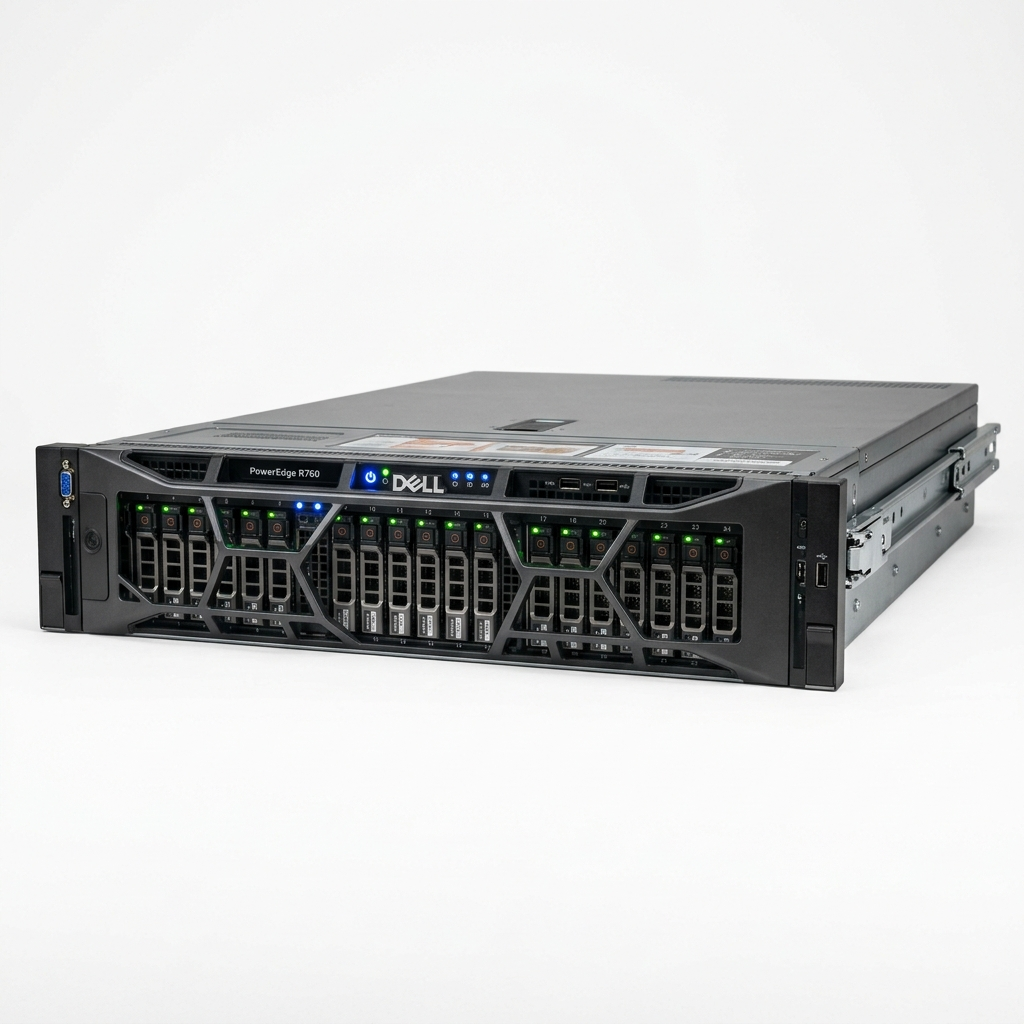
\includegraphics[width=0.6\textwidth]{dell_poweredge_server.png}
			\caption{Dell PowerEdge R760 5G Core Server (Procured via Dell India / ServerBasket)}
			\label{fig}
		\end{figure}
		
		\newpage
		
		\subsection{Module 3: AI and Mobility Controller Workstation}The AI layer hosts the DNN-based slice selection algorithms, traffic prediction models, and deep reinforcement learning (DRL) agents. Training and running these models in real time during handover events requires high VRAM and parallel compute capabilities.
		\begin{itemize}
			\item \textbf{Compute:} Intel Core i9-14900K with 64GB DDR5 RAM.
			\item \textbf{Accelerator:} NVIDIA GeForce RTX 4090 with 24GB GDDR6X VRAM, optimized for CUDA and TensorRT inference.
			\item \textbf{Cooling:} Custom closed-loop liquid cooling system to prevent thermal throttling during continuous training cycles.
		\end{itemize}
		 shows the physical design of the liquid-cooled AI workstation, featuring multiple GPU configurations and custom cooling tubes.
		
		\begin{figure}[htbp]
			\centering
			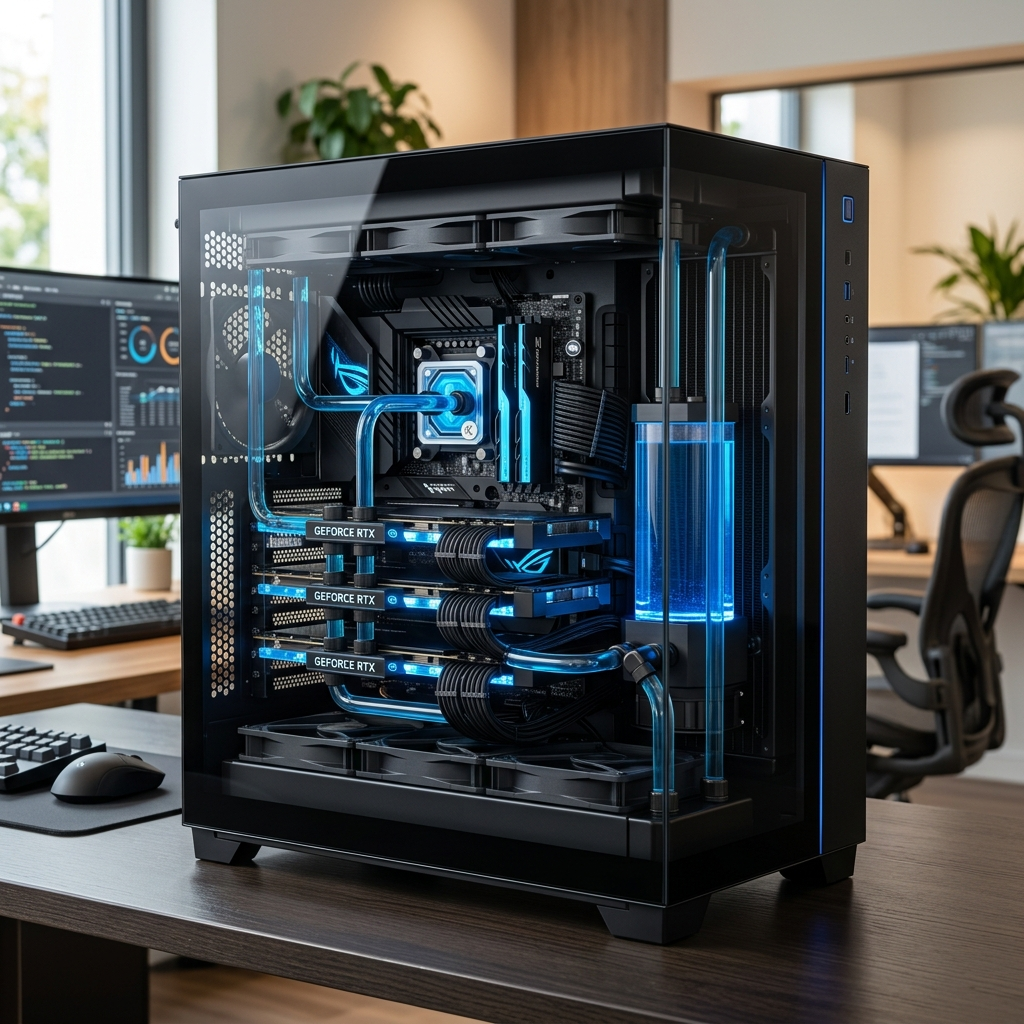
\includegraphics[width=0.6\textwidth]{gpu_ai_workstation.png}
			\caption{High-Performance Liquid-Cooled AI GPU Workstation (Procured via Volted PC / PC Kumar)}
			\label{fig}
		\end{figure}
		
		\subsection{Module 4: Central Storage NAS Chassis}Network logs, Wireshark packet captures (PCAPs), and telemetry metrics from Grafana/Prometheus must be centralized and backed up for training dataset creation. This is handled by a high-availability network storage unit.
		\begin{itemize}
			\item \textbf{Model:} Synology DS1821+ (8-Bay Desktop NAS).
			\item \textbf{Storage:} 4 $\times$ 4TB Seagate IronWolf NAS-grade SATA HDDs configured in RAID 5.
			\item \textbf{Expansion:} Built-in PCIe slot populated with a dual-port 10GbE card for high-speed file transfers.
		\end{itemize}
		 displays the front and rear panels of the Synology DS1821+ NAS unit.
		
		\begin{figure}[htbp]
			\centering
			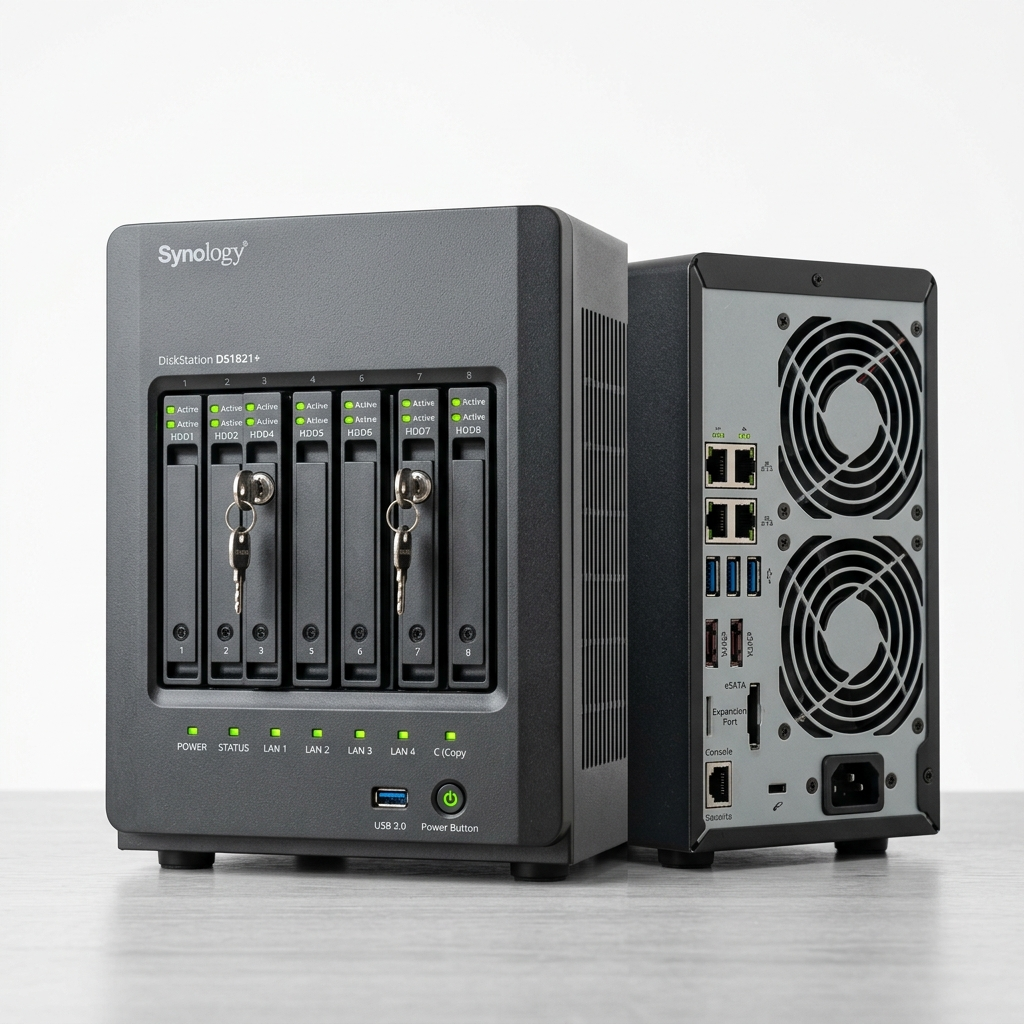
\includegraphics[width=0.6\textwidth]{synology_nas_storage.png}
			\caption{Synology DS1821+ 8-Bay NAS Chassis (Procured via Computech / Vishal Peripherals)}
			\label{fig}
		\end{figure}
		
		\newpage
		
		\section{Software Stack Integration Plan}The testbed leverages standard open-source cellular stacks integrated with standard container orchestration.  outlines the software layers implemented across the physical servers.
		
		\begin{itemize}
			\item \textbf{5G Core Network (Open5GS):} Provides AMF (Access and Mobility Management), SMF (Session Management), UPF (User Plane Function), UDM (Unified Data Management), and AUSF (Authentication Server Function). It uses MongoDB to store subscriber profiles (SIM details, slice subscription, keys).
			\item \textbf{Radio Access Network (srsRAN Project):} Instantiates a software-based gNodeB that interfaces with the USRP B210 via the UHD (USRP Hardware Driver) API. It supports split-8 PHY/MAC layers.\textbf{Edge Computing Platform (Kubernetes/Docker):} Deployed on the MEC server to manage containerized edge services. KubeEdge or custom load-balancers redirect traffic dynamically during handovers.
			\item \textbf{Telemetry Stack (Prometheus \& Grafana):} Continuously queries cellular KPIs (e.g., active UEs, bandwidth per slice, packet latency, jitter, RSRP, and drop rates) using custom exporters on Open5GS and srsRAN.\end{itemize}
		
		\begin{figure}[htbp]
			\centering
			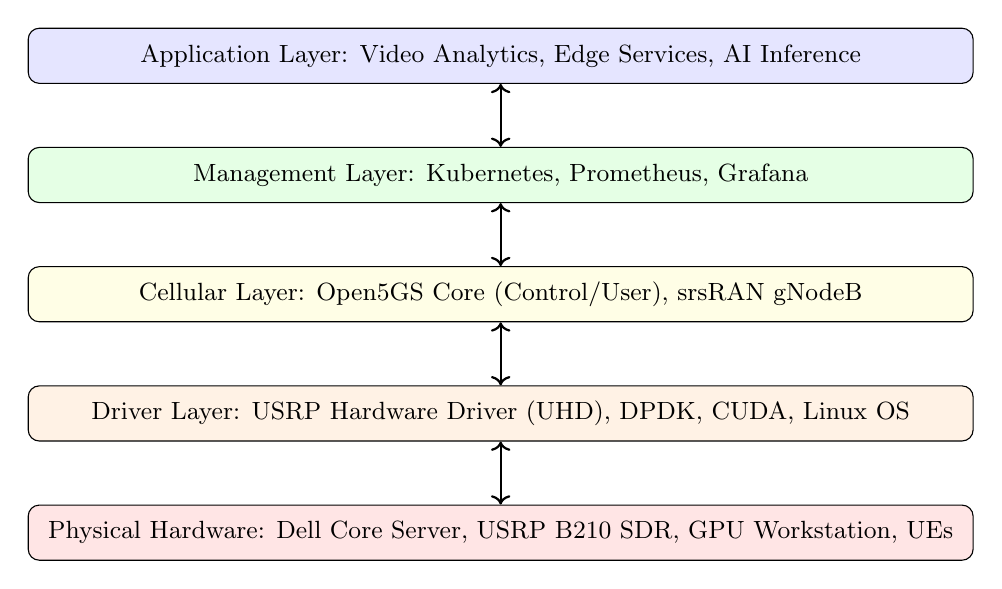
\begin{tikzpicture}
				[every node/.style={draw, rounded corners, align=center, minimum width=12cm, minimum height=0.7cm, font=\small},node distance=0.8cm]\node (app) [fill=blue!10] {Application Layer: Video Analytics, Edge Services, AI Inference};\node (mgmt) [below=of app, fill=green!10] {Management Layer: Kubernetes, Prometheus, Grafana};\node (telephony) [below=of mgmt, fill=yellow!10] {Cellular Layer: Open5GS Core (Control/User), srsRAN gNodeB};\node (drivers) [below=of telephony, fill=orange!10] {Driver Layer: USRP Hardware Driver (UHD), DPDK, CUDA, Linux OS};\node (hw) [below=of drivers, fill=red!10] {Physical Hardware: Dell Core Server, USRP B210 SDR, GPU Workstation, UEs};
				
				\draw[<->, thick] (app) -- (mgmt);
				\draw[<->, thick] (mgmt) -- (telephony);
				\draw[<->, thick] (telephony) -- (drivers);
				\draw[<->, thick] (drivers) -- (hw);
			\end{tikzpicture}
			\caption{5G Testbed Integrated Software Stack}
			\label{fig:software_stack}
			
		\end{figure}
		
		\section{Junior Research Fellow (JRF) Profile}A Junior Research Fellow (JRF) will be recruited to support the installation, integration, and day-to-day operation of the 5G testbed.
		
		\subsection{Essential Technical Qualifications}\begin{itemize}\item B.Tech/M.Tech in Computer Science, Electronics \& Communication, or Information Technology.\item \textbf{Linux Systems Administration:} Experience with Ubuntu Server, systemd, bash scripting, network interface configurations (IP routing, VLANs, bridging).\item \textbf{Programming:} Proficiency in Python and C/C++.\item \textbf{Networking Fundamentals:} Deep understanding of the TCP/IP stack, routing protocols, sockets, and network analysis tools (Wireshark, tcpdump).\end{itemize}
		
		\subsection{Desirable Technical Qualifications}\begin{itemize}\item GATE qualification in CS or EC.\item Hands-on experience compiling and configuring Open5GS, srsRAN, or OpenAirInterface.\item Familiarity with Software-Defined Radio (SDR) hardware and UHD library.\item Knowledge of Docker, Kubernetes, and containerized deployment patterns.\item Basic understanding of machine learning frameworks (PyTorch or TensorFlow).\end{itemize}
		
		\section{Risk Assessment \& Mitigation Plan}Table~\ref{tab} lists potential technical and logistical risks associated with the implementation of the 5G testbed, along with corresponding mitigation strategies.
		
	\begin{table}[htbp]
		\centering
		\caption{Project Risk Assessment and Mitigation Matrix}
		\label{tab:risk_assessment}
		
		\begin{tabular}{
				p{3.3cm}
				p{2.2cm}
				p{9.0cm}
			}
			
			\toprule
			
			\textbf{Risk Event} &
			\textbf{Impact Level} &
			\textbf{Mitigation Strategy} \\
			
			\midrule
			
			Procurement Delays &
			Medium &
			Utilize pre-approved Indian distributors (GSAS India, Dell India, HPE India) to minimize customs clearance delays and ensure timely delivery. \\
			
			\addlinespace
			
			SDR Hardware Overheating &
			Medium &
			Install active cooling fans on the USRP B210 enclosures, provide adequate ventilation, and limit continuous high-power transmission during prolonged experiments. \\
			
			\addlinespace
			
			RF Interference &
			High &
			Conduct initial experiments using RF coaxial cables with programmable attenuators before transitioning to over-the-air testing. Employ spectrum analysis to identify and mitigate interference sources. \\
			
			\addlinespace
			
			Core Network Configuration Errors &
			High &
			Maintain version-controlled configuration files, periodic VM snapshots, Docker container backups, and automated health checks for rapid recovery. \\
			
			\addlinespace
			
			UPS Battery Failure &
			Low &
			Establish preventive maintenance contracts with the UPS vendor, perform periodic battery health monitoring, and configure graceful server shutdown using network-enabled UPS management. \\
			
			\bottomrule
			
		\end{tabular}
		
	\end{table}
		
	\end{document}